\section{Background}
Maintenance scheduling is a combinatorial optimisation problem with $T^N$ assignments for $N$ machines and $T$ time slots, subject to capacity and assignment constraints. MILP guarantees optimality but scales poorly on large instances. This chapter benchmarks three paradigms against the classical baseline: quantum-inspired heuristics on classical hardware, gate-based QAOA on IBM Quantum hardware, and exact MILP/CBC for reference.

\section{Problem Formulation}
\subsection{Maintenance Scheduling as Combinatorial Optimization}
Each of $N$ machines is assigned to one of $T$ discrete slots within a 72-hour horizon (slot size $s = 72/T$~h). Machine $i$ has priority score $p_i \in [0,100]$ from upstream anomaly and damage estimation. The objective is
\begin{equation}
\min_{ \{t_i\}_{i=1}^N }
\sum_{i=1}^{N}
\left[ C_{\text{maint}}
+ C_{\text{risk}} \cdot \frac{p_i}{100} \cdot \frac{t_i}{H} \right],
\end{equation}
with $C_{\text{maint}}=100$, $C_{\text{risk}}=1000$. A machine with $p_i=90$ at $t_i=36$ incurs $100 + 1000 \cdot 0.9 \cdot 36/72 = 550$ versus only $100$ at $t_i=0$, so the formulation penalises delayed scheduling of high-priority machines.

\subsection{Constraints}
Two hard constraints govern feasibility. \textbf{(1) One-hot:} each machine occupies exactly one slot,
\begin{equation}
\sum_{j=1}^{T} x_{i,j} = 1, \quad \forall i \in \{1, \ldots, N\},
\end{equation}
with $x_{i,j} \in \{0,1\}$ indicating machine $i$ in slot $j$. \textbf{(2) Capacity:} at most $C=3$ machines run concurrently per slot,
\begin{equation}
\sum_{i=1}^{N} x_{i,j} \leq C, \quad \forall j \in \{1, \ldots, T\}.
\end{equation}
These reflect crew, spare-parts, and safety limits.

\subsection{Time Discretization}
$T$ is set adaptively to keep the feasible region from collapsing at $N = C T$:
\begin{equation}
T = \max\!\left(4,\; \left\lceil \frac{N}{C} \right\rceil + \max\!\left(1,\; \left\lfloor \frac{N}{10} \right\rfloor \right) \right).
\end{equation}
The slack $\max(1,\lfloor N/10 \rfloor)$ expands the feasible region beyond the minimum $\lceil N/C \rceil$ slots.

\subsection{Detailed Constraint Specification}
\label{sec:constraint_specification}

The complex-constraint MILP, complex QUBO, and feasibility-aware metaheuristics of Section~\ref{sec:metaheuristics} share four hard constraints. Let $x_{i,j} \in \{0,1\}$ be $1$ iff machine $i$ \emph{starts} in slot $j$:
\begin{align}
\textbf{(C1) one-hot:} \quad &
\sum_{j=0}^{T-1} x_{i,j} = 1, \quad \forall i.
\\
\textbf{(C2) slot-window capacity:} \quad &
\sum_{i=1}^{N} \sum_{\,j' = \max(0, j-d+1)}^{j} x_{i,j'} \leq C,
\quad \forall j.
\\
\textbf{(C3) risk horizon:} \quad &
\sum_{j=0}^{\rho - 1} x_{i,j} \geq 1, \quad
\forall i \in \mathcal{R}, \notag \\
& \mathcal{R} = \{ i : \mathrm{risk\_state}_i \,\vee\,
  \mathrm{priority\_level}_i \in \{\mathrm{C, H}\}\}, \notag \\
\textbf{(C4) must-schedule:} \quad &
\text{every } i \text{ with } \mathrm{needs\_maint}_i\!=\!1 \text{ enters (C1)}. \notag
\end{align}
With $d=4$ h, $C=3$, $\rho = \max(1, \lfloor 24 / s \rfloor)$ slots (matching Chapter~5 operational parameters), (C2) counts capacity over the \emph{active} $d$-slot window so that maintenance still in progress at slot $j$ contributes to that slot's capacity, and (C3) forces every CRITICAL/HIGH machine to start within the operator-defined deadline of the first $\rho$ slots. The streaming pipeline of Section~\ref{sec:complex_streaming} runs every solver against (C1)--(C4) for an honest, real-deployment comparison; the basic-constraint variant of Section~\ref{sec:scaling_benchmark_basic} keeps only (C1) plus slot-level capacity for synthetic ablation.

\section{Quadratic Unconstrained Binary Optimization}
Quantum-inspired and gate-based quantum solvers require a QUBO formulation
\begin{equation}
\min_{\mathbf{x} \in \{0,1\}^n} \; \mathbf{x}^\top \mathbf{Q} \mathbf{x},
\end{equation}
with $n = N T$ binary variables and a symmetric matrix $\mathbf{Q}$ that encodes both objective and constraints (the latter as quadratic penalties).

\subsection{Objective Encoding}
The scheduling cost lands on the diagonal:
\begin{equation}
Q_{(i,j),(i,j)} \mathrel{+}=
C_{\text{maint}} + C_{\text{risk}} \cdot \frac{p_i}{100} \cdot \frac{j}{T},
\end{equation}
exploiting $x_{i,j}^2 = x_{i,j}$ for binary variables to map the linear objective into quadratic form.

\subsection{Constraint Encoding via Penalty Terms}
\textbf{One-hot.} $\lambda_{\text{assign}} (\sum_j x_{i,j} - 1)^2$ expands via $x_j^2 = x_j$ to $-\sum_j x_j + 2\sum_{j<k} x_j x_k + 1$, contributing
\begin{align}
Q_{(i,j),(i,j)} \mathrel{+}= -\lambda_{\text{assign}}, \quad
Q_{(i,j),(i,k)} \mathrel{+}= 2\lambda_{\text{assign}}\;(j<k).
\end{align}
\textbf{Capacity.} Pairwise co-assignment in the same slot is penalised:
\begin{equation}
Q_{(i_1,j),(i_2,j)} \mathrel{+}= \lambda_{\text{cap}} / C, \quad \forall i_1 \neq i_2.
\end{equation}

\subsection{Penalty Weight Calibration}
Weights are derived from the problem parameters rather than hand-tuned. With
\begin{equation}
C_{\max} = C_{\text{maint}} + C_{\text{risk}} \cdot \max_i p_i / 100,
\end{equation}
we set $\lambda_{\text{assign}} = 3 \cdot C_{\max} \cdot T$ and $\lambda_{\text{cap}} = 2 \cdot C_{\max}$. The factor 3 ensures the one-hot penalty dominates any objective gain from leaving a machine unscheduled, so the search cannot trade constraint violations for lower cost.

\begin{algorithm}[!htbp]
\small
\caption{Build QUBO Matrix for Scheduling}
\label{alg:build_qubo}
\begin{algorithmic}[1]
\Require machines with priorities $\{p_i\}_{i=1}^N$, time slots $T$, capacity $C$, costs $(c_{\text{maint}}, c_{\text{risk}})$
\Ensure symmetric QUBO matrix $\mathbf{Q} \in \mathbb{R}^{n \times n}$, where $n = N \cdot T$
\State $n \gets N \cdot T$
\State $\mathbf{Q} \gets \mathbf{0}_{n \times n}$
\Statex \textbf{// Compute data-driven penalty weights}
\State $p_{\max} \gets \max_i \left( \frac{p_i}{100} \right)$
\State $C_{\max} \gets c_{\text{maint}} + c_{\text{risk}} \cdot p_{\max}$
\State $\lambda_{\text{assign}} \gets 3 \cdot C_{\max} \cdot T$
\State $\lambda_{\text{cap}} \gets 2 \cdot C_{\max}$
\Statex \textbf{// Encode scheduling cost on diagonal}
\For{$i = 0$ to $N-1$}
    \For{$j = 0$ to $T-1$}
        \State $k \gets i \cdot T + j$
        \State $Q_{k,k} \gets Q_{k,k} + c_{\text{maint}} + c_{\text{risk}} \cdot \frac{p_i}{100} \cdot \frac{j}{T}$
    \EndFor
\EndFor
\Statex \textbf{// One-hot constraint: $(\sum_j x_{i,j} - 1)^2$}
\For{$i = 0$ to $N-1$}
    \For{$j = 0$ to $T-1$}
        \State $k \gets i \cdot T + j$
        \State $Q_{k,k} \gets Q_{k,k} - \lambda_{\text{assign}}$
    \EndFor
    \For{$j = 0$ to $T-1$}
        \For{$\ell = j+1$ to $T-1$}
            \State $k_1 \gets i \cdot T + j$
            \State $k_2 \gets i \cdot T + \ell$
            \State $Q_{k_1,k_2} \gets Q_{k_1,k_2} + 2 \cdot \lambda_{\text{assign}}$
        \EndFor
    \EndFor
\EndFor
\Statex \textbf{// Capacity constraint: penalise same-slot co-assignment}
\For{$j = 0$ to $T-1$}
    \For{$i_1 = 0$ to $N-1$}
        \For{$i_2 = i_1+1$ to $N-1$}
            \State $k_1 \gets i_1 \cdot T + j$
            \State $k_2 \gets i_2 \cdot T + j$
            \State $Q_{k_1,k_2} \gets Q_{k_1,k_2} + \frac{\lambda_{\text{cap}}}{C}$
        \EndFor
    \EndFor
\EndFor
\Statex \textbf{// Symmetrize matrix}
\State $\mathbf{Q} \gets (\mathbf{Q} + \mathbf{Q}^\top)/2$
\State \Return $\mathbf{Q}$
\end{algorithmic}
\end{algorithm}

\subsection{QUBO to Ising Conversion}
For quantum annealing-based methods (e.g., SQA) and gate-based quantum algorithms (e.g., QAOA), the QUBO formulation is transformed into an equivalent Ising Hamiltonian using the substitution:
\begin{equation}
x_i = \frac{1 + \sigma_i}{2}, \quad \sigma_i \in \{-1, +1\}.
\end{equation}

Under this transformation, the QUBO objective can be expressed as an Ising Hamiltonian:
\begin{equation}
H_{\text{Ising}} = \sum_{i} h_i \, \sigma_i + \sum_{i<j} J_{i,j} \, \sigma_i \sigma_j + \text{offset}.
\end{equation}

The corresponding coefficients are given by:
\begin{align}
h_i &= \frac{Q_{i,i}}{2} + \sum_{j \neq i} \frac{Q_{i,j}}{4}, \\
J_{i,j} &= \frac{Q_{i,j}}{4}, \\
\text{offset} &= \sum_{i} \frac{Q_{i,i}}{4} + \sum_{i<j} \frac{Q_{i,j}}{4}.
\end{align}

\section{Quantum-Inspired Algorithms}
Quantum-inspired algorithms are classical algorithms that incorporate heuristics motivated by quantum mechanical principles. They execute on standard hardware in polynomial time and space, without simulating quantum mechanics. Two algorithms are implemented: the Quantum-Inspired Evolutionary Algorithm (QIEA) and Simulated Quantum Annealing (SQA).

\subsubsection{Quantum-Inspired Evolutionary Algorithm (QIEA)}
QIEA \cite{HanKim2002} represents candidate solutions using quantum probability amplitudes rather than classical bitstrings. Each individual in the population is a vector of qubit states:
\begin{equation}
\lvert \psi_i \rangle = \alpha_i \lvert 0 \rangle + \beta_i \lvert 1 \rangle, 
\quad \text{where } \alpha_i^2 + \beta_i^2 = 1.
\end{equation}

The algorithm maintains a population of K such quantum individuals, each encoding a probability distribution over the n-bit decision space.
Observation. At each generation, classical bitstrings are sampled from the amplitude distribution. For each bit i, the observed value is 1 with probability beta$_i^2$ and 0 with probability $alpha_i^2$. This sampling is vectorized for efficiency: probabilities are computed as a K x n matrix, compared against uniform random values, yielding K observed classical solutions per generation.
Evaluation. Each observed bitstring x is evaluated by computing $x^T$ Q x (QUBO energy). The best solution found across all generations is maintained.
Quantum rotation gate update. After evaluation, the Q-gate angles are rotated toward the best-known solution:

\begin{equation}
\Delta \theta = 0.01 \pi \cdot \max\!\left(0.1,\; 1 - \frac{g}{G}\right)
\end{equation}

where g is the current generation and G is the total number of generations. The rotation sign depends on the relationship between the current amplitude bias and the target bit value. This annealing-like schedule reduces the rotation magnitude over time, transitioning from exploration to exploitation. \textbf{Adaptive scaling}. Population size and generation count scale with the problem dimension:
\begin{align}
K &= \max\!\left(20,\; \min\!\left(50,\; \frac{n_{\text{bits}}}{4}\right)\right), \\
G &= \max\!\left(200,\; \min\!\left(400,\; n_{\text{bits}}\right)\right).
\end{align}

This prevents both under-exploration for large problems and wasteful computation for small ones.

\begin{algorithm}[!htbp]
\small
\caption{Quantum-Inspired Evolutionary Algorithm (QIEA) for QUBO Optimisation}
\label{alg:qiea}
\begin{algorithmic}[1]
\Require QUBO matrix $\mathbf{Q} \in \mathbb{R}^{n \times n}$, number of variables $n = N \cdot T$, number of machines $N$, number of time slots $T$
\Ensure Best solution $\mathbf{x}^*$ and energy $E^*$
\Statex \textbf{// Adaptive parameter scaling}
\State $K \gets \max\!\left(20,\; \min\!\left(50,\; \left\lfloor \frac{n}{4} \right\rfloor \right)\right)$
\State $G \gets \max\!\left(200,\; \min\!\left(400,\; n \right)\right)$
\Statex \textbf{// Initialise quantum population}
\For{$k = 0$ to $K-1$}
    \For{$i = 0$ to $n-1$}
        \State $\alpha_{k,i} \gets \frac{1}{\sqrt{2}}$
        \State $\beta_{k,i} \gets \frac{1}{\sqrt{2}}$
    \EndFor
\EndFor
\State $\mathbf{x}^* \gets \emptyset$, \quad $E^* \gets +\infty$
\Statex
\For{$g = 0$ to $G-1$}
    \Statex \textbf{// Step 1: Observation}
    \For{$k = 0$ to $K-1$}
        \For{$i = 0$ to $n-1$}
            \State $r \sim \mathcal{U}(0,1)$
            \State $x_{k,i} \gets 
            \begin{cases}
            1, & r < \beta_{k,i}^2 \\
            0, & \text{otherwise}
            \end{cases}$
        \EndFor
    \EndFor
    \Statex \textbf{// Step 2: Evaluation}
    \For{$k = 0$ to $K-1$}
        \State $E_k \gets \mathbf{x}_k^\top \mathbf{Q} \mathbf{x}_k$
        \If{$E_k < E^*$}
            \State $E^* \gets E_k$
            \State $\mathbf{x}^* \gets \mathbf{x}_k$
        \EndIf
    \EndFor
    \Statex \textbf{// Step 3: Update (Q-gate rotation)}
    \State $\Delta \theta \gets 0.01\pi \cdot \max\!\left(0.1,\; 1 - \frac{g}{G}\right)$
    \For{$k = 0$ to $K-1$}
        \For{$i = 0$ to $n-1$}
            \If{$x_{k,i} = x^*_i$}
                \State \textbf{continue}
            \EndIf
            \If{$x^*_i = 1$}
                \State $\text{sign} \gets 
                \begin{cases}
                +1, & \alpha_{k,i} \beta_{k,i} > 0 \\
                -1, & \text{otherwise}
                \end{cases}$
            \Else
                \State $\text{sign} \gets 
                \begin{cases}
                -1, & \alpha_{k,i} \beta_{k,i} > 0 \\
                +1, & \text{otherwise}
                \end{cases}$
            \EndIf
            \State $\delta \gets \text{sign} \cdot \Delta \theta$
            \State $\alpha'_{k,i} \gets \cos(\delta)\,\alpha_{k,i} - \sin(\delta)\,\beta_{k,i}$
            \State $\beta'_{k,i} \gets \sin(\delta)\,\alpha_{k,i} + \cos(\delta)\,\beta_{k,i}$
            \State $\alpha_{k,i} \gets \alpha'_{k,i}$
            \State $\beta_{k,i} \gets \beta'_{k,i}$
        \EndFor
    \EndFor
\EndFor
\State \Return $\mathbf{x}^*, E^*$
\end{algorithmic}
\end{algorithm}

The rotation gate (lines 45–49) is the core quantum-inspired mechanism. Unlike classical genetic algorithms that rely on crossover and mutation, QIEA evolves the probability distribution over solutions. The annealing schedule on Δθ (line 34) ensures broad exploration in early generations (large rotations) and fine-tuning in later generations (small rotations), analogous to the temperature schedule in simulated annealing but operating in the amplitude space.

\section{Simulated Quantum Annealing (SQA)}
SQA \cite{KadowakiNishimori1998} simulates quantum annealing using path-integral Monte Carlo. The quantum system with transverse field is mapped to a classical system with an additional (imaginary time) dimension via the Suzuki-Trotter decomposition. The algorithm maintains M = 16 classical replicas (Trotter slices) coupled by an inter-replica interaction:

\begin{equation}
J_{\perp} = -\frac{T_{\text{phys}}}{2} \, \ln\!\left( \tanh\!\left( \frac{\Gamma}{M \, T_{\text{phys}}} \right) \right)
\end{equation}

where Gamma is the transverse field strength and $T_phys$ is the physical temperature.

\textbf{Annealing schedule.} The transverse field Gamma decreases linearly from $Gamma_start$ = 5.0 to $Gamma_end$ = 0.01 over S sweeps. At each sweep, single-spin Metropolis updates are proposed for each spin in each replica. The acceptance criterion accounts for both the problem Hamiltonian energy change and the inter-replica coupling:

\begin{equation}
\Delta E = 2 \, \sigma_i \left[
h_i + \sum_{j} J_{i,j} \, \sigma_j + J_{\perp} \left( \sigma_i^{k-1} + \sigma_i^{k+1} \right)
\right]
\end{equation}

where $sigma_i^{k-1}$ and $sigma_i^{k+1}$ are the spin values in adjacent replicas. The flip is accepted if $Delta_E$ < 0 or with probability $exp(-Delta_E / T_phys)$. \textbf{Sweep scaling}. The number of sweeps adapts to problem size:

\begin{equation}
S = \min\!\left(500,\; \max\!\left(200,\; \frac{500 \cdot 20}{n_{\text{bits}}}\right)\right)
\end{equation}

This caps computation time for large instances while maintaining sufficient sampling for small ones.

The key distinction between SQA and classical simulated annealing lies in the inter-replica coupling term (lines 30–32). The M replicas interact through $J_⊥$, which encodes the effect of quantum tunneling in the Suzuki-Trotter decomposition. When Γ is large, $J_⊥$ is strong and replicas are tightly coupled (high quantum fluctuations); as Γ → 0, $J_⊥$ → 0 and replicas decouple, each converging independently to a classical minimum. The random permutation at line 19 prevents systematic bias in the sweep order.

\section{Gate-Based Quantum Optimization (QAOA)}
\subsection{QAOA with XY Ring Mixer}
The Quantum Approximate Optimization Algorithm \cite{Farhi2014} constructs a parameterized quantum circuit that alternates between a problem unitary and a mixing unitary. The standard QAOA uses a transverse-field mixer (sum of X gates), which does not respect the one-hot constraint. Following Hadfield et al.\ \cite{Hadfield2019}, we employ an XY ring mixer that structurally preserves the Hamming weight within each machine's qubit block.

\begin{algorithm}[!htbp]
\small
\caption{QAOA with XY Mixer for Scheduling}
\label{alg:qaoa_xy}
\begin{algorithmic}[1]
\Require local fields $\mathbf{h}$, couplings $\mathbf{J}$, machines $N$, time slots $T$, layers $p$, restarts $R$, max iterations $I$
\Ensure best feasible solution $\mathbf{x}^*$ and cost $C^*$
\State $n \gets N \cdot T$
\State $\text{dim} \gets 2^n$
\Statex \textbf{// Precompute Ising Hamiltonian diagonal}
\For{$z = 0$ to $\text{dim}-1$}
    \State $\boldsymbol{\sigma} \gets \text{spin\_vector}(z, n)$
    \State $H_{\text{diag}}[z] \gets \sum_i h_i \sigma_i + \sum_{i<j} J_{i,j} \sigma_i \sigma_j$
\EndFor
\Statex \textbf{// Initial state: one-hot per machine}
\State $\lvert \psi_{\text{init}} \rangle \gets \bigotimes_{m=1}^{N} \lvert 10\ldots 0 \rangle$
\State $\gamma^* \gets \emptyset$, \quad $\boldsymbol{\beta}^* \gets \emptyset$, \quad $C^* \gets +\infty$
\Statex
\For{$r = 0$ to $R-1$}
    \State $(\boldsymbol{\gamma}_0, \boldsymbol{\beta}_0) \gets \text{random initial angles in } \mathbb{R}^p \times \mathbb{R}^p$
    \Statex \textbf{// Define cost function}
    \Function{QAOA\_Cost}{$\boldsymbol{\gamma}, \boldsymbol{\beta}$}
        \State $\lvert \psi \rangle \gets \lvert \psi_{\text{init}} \rangle$
        \For{$\ell = 0$ to $p-1$}
            \State $\lvert \psi \rangle \gets e^{-i \gamma_\ell H_{\text{diag}}} \lvert \psi \rangle$
            \For{$m = 0$ to $N-1$}
                \For{$t = 0$ to $T-1$}
                    \State $q_a \gets m \cdot T + t$
                    \State $q_b \gets m \cdot T + (t+1) \bmod T$
                    \State Apply XY($\beta_\ell$) on $(q_a, q_b)$:
                    \Statex \hspace{2em}
                    $\lvert 01 \rangle \rightarrow \cos(\beta_\ell)\lvert 01 \rangle - i\sin(\beta_\ell)\lvert 10 \rangle$
                    \Statex \hspace{2em}
                    $\lvert 10 \rangle \rightarrow -i\sin(\beta_\ell)\lvert 01 \rangle + \cos(\beta_\ell)\lvert 10 \rangle$
                \EndFor
            \EndFor
        \EndFor
        \State \Return $\sum_z |\langle z | \psi \rangle|^2 \cdot H_{\text{diag}}[z]$
    \EndFunction
    \State $(\boldsymbol{\gamma}_{\text{opt}}, \boldsymbol{\beta}_{\text{opt}}) \gets \text{COBYLA}(\text{QAOA\_Cost}, (\boldsymbol{\gamma}_0, \boldsymbol{\beta}_0), I)$
    \If{$\text{QAOA\_Cost}(\boldsymbol{\gamma}_{\text{opt}}, \boldsymbol{\beta}_{\text{opt}}) < C^*$}
        \State $C^* \gets \text{QAOA\_Cost}(\boldsymbol{\gamma}_{\text{opt}}, \boldsymbol{\beta}_{\text{opt}})$
        \State $\boldsymbol{\gamma}^* \gets \boldsymbol{\gamma}_{\text{opt}}$
        \State $\boldsymbol{\beta}^* \gets \boldsymbol{\beta}_{\text{opt}}$
    \EndIf
\EndFor
\Statex \textbf{// Sampling best solution}
\State $\lvert \psi_{\text{final}} \rangle \gets \text{QAOA}(\boldsymbol{\gamma}^*, \boldsymbol{\beta}^*)$
\State $p(z) \gets |\langle z | \psi_{\text{final}} \rangle|^2$
\State $\mathbf{x}^* \gets \emptyset$, \quad $\text{Cost}^* \gets +\infty$
\For{top $200$ states $z$ sorted by $p(z)$}
    \State $\mathbf{x} \gets \text{binary\_vector}(z, n)$
    \State feasible $\gets$ true
    \For{$m = 0$ to $N-1$}
        \If{$\sum_{j=0}^{T-1} x_{mT+j} \neq 1$}
            \State feasible $\gets$ false
        \EndIf
    \EndFor
    \If{feasible \textbf{and} $\text{PureCost}(\mathbf{x}) < \text{Cost}^*$}
        \State $\text{Cost}^* \gets \text{PureCost}(\mathbf{x})$
        \State $\mathbf{x}^* \gets \mathbf{x}$
    \EndIf
\EndFor
\State \Return $\mathbf{x}^*, \text{Cost}^*$
\end{algorithmic}
\end{algorithm}

The critical insight in Algorithm \ref{alg:qaoa_xy}  is that the XY ring mixer (lines 28–37) operates within each machine's qubit block, swapping amplitude only between basis states that have the same Hamming weight. Starting from a one-hot initial state (line 11), the mixer can only reach other one-hot configurations, eliminating the need for the one-hot penalty term during the quantum search and preserving feasibility by construction. This contrasts with QIEA and SQA, which must enforce one-hot constraints through penalty terms in the QUBO energy.

\begin{algorithm}[!htbp]
\small
\caption{QAOA Hardware Execution Pipeline}
\label{alg:qaoa_hardware}
\begin{algorithmic}[1]
\Require machines $\mathcal{M}$, time slots $T$, API token, quantum backend
\Ensure best feasible solution $\mathbf{x}^*$ and cost $\text{Cost}^*$
\Statex \textbf{// Phase 1: Parameter optimisation on reduced problem}
\State $N_{\text{opt}} \gets \min(N, 4)$
\State $\mathcal{M}_{\text{opt}} \gets \mathcal{M}[0 : N_{\text{opt}}]$
\State $(\mathbf{h}_{\text{opt}}, \mathbf{J}_{\text{opt}}) \gets \text{BuildQUBO} \rightarrow \text{Ising}(\mathcal{M}_{\text{opt}}, T)$
\State $(\boldsymbol{\gamma}^*, \boldsymbol{\beta}^*) \gets \text{QAOA-XY}(\mathbf{h}_{\text{opt}}, \mathbf{J}_{\text{opt}}, N_{\text{opt}}, T, p, \text{restarts}, \text{max\_iter})$
\Statex \textbf{// Phase 2: Build parameterised circuit}
\State $n_{\text{qubits}} \gets N \cdot T$
\State $qc \gets \text{QuantumCircuit}(n_{\text{qubits}})$
\For{$m = 0$ to $N-1$}
    \State $qc.x(m \cdot T)$
\EndFor
\State $(\mathbf{h}_{\text{full}}, \mathbf{J}_{\text{full}}) \gets \text{BuildQUBO} \rightarrow \text{Ising}(\mathcal{M}, T)$
\For{$\ell = 0$ to $p-1$}
    \Statex \textbf{// Problem unitary}
    \For{$i = 0$ to $n_{\text{qubits}}-1$}
        \State $qc.\text{rz}(2 \gamma^*_\ell \, h_{\text{full}}[i],\; i)$
    \EndFor
    \For{all $(i,j)$ with $J_{\text{full}}[i,j] \neq 0$}
        \State $qc.\text{cx}(i, j)$
        \State $qc.\text{rz}(2 \gamma^*_\ell \, J_{\text{full}}[i,j],\; j)$
        \State $qc.\text{cx}(i, j)$
    \EndFor
    \Statex \textbf{// XY ring mixer}
    \For{$m = 0$ to $N-1$}
        \For{$t = 0$ to $T-1$}
            \State $q_a \gets m \cdot T + t$
            \State $q_b \gets m \cdot T + (t+1) \bmod T$
            \State $qc.\text{cx}(q_a, q_b)$
            \State $qc.\text{ry}(2 \beta^*_\ell, q_a)$
            \State $qc.\text{cx}(q_b, q_a)$
            \State $qc.\text{ry}(-2 \beta^*_\ell, q_a)$
            \State $qc.\text{cx}(q_a, q_b)$
        \EndFor
    \EndFor
\EndFor
\State $qc.\text{measure\_all}()$
\Statex \textbf{// Phase 3: Execute on hardware}
\State $qc_t \gets \text{transpile}(qc, \text{backend}, \text{optimization\_level}=3)$
\State job $\gets \text{SamplerV2}(\text{backend}).\text{run}(qc_t, \text{shots}=4096)$
\State counts $\gets \text{job.result}()$
\Statex \textbf{// Phase 4: Decode and select solution}
\State $\mathbf{x}^* \gets \emptyset$, \quad $\text{Cost}^* \gets +\infty$
\For{each $(\text{bitstring}, \text{count})$ in counts}
    \State $\mathbf{x} \gets \text{decode}(\text{bitstring})$
    \If{$\text{is\_one\_hot}(\mathbf{x}, N, T)$ \textbf{and} $\text{is\_capacity\_ok}(\mathbf{x})$}
        \If{$\text{PureCost}(\mathbf{x}) < \text{Cost}^*$}
            \State $\text{Cost}^* \gets \text{PureCost}(\mathbf{x})$
            \State $\mathbf{x}^* \gets \mathbf{x}$
        \EndIf
    \EndIf
\EndFor
\State \Return $\mathbf{x}^*, \text{Cost}^*$
\end{algorithmic}
\end{algorithm}

Algorithm \ref{alg:qaoa_hardware} addresses the key practical challenge of QAOA on NISQ hardware: the variational optimization loop is prohibitively expensive when executed on-device. The parameter transfer strategy (lines 1–5) optimizes angles on a classically simulable sub-problem, then applies them to the full-size circuit. This assumes concentration of QAOA parameters — that optimal angles for small instances generalize to larger instances of the same problem class \cite{Brandao2018}. The transpilation step (line 43) maps the abstract circuit to the hardware's native gate set and qubit connectivity, introducing SWAP gates that increase circuit depth.
Figure 7 illustrates the circuit architecture for a minimal instance (N = 2 machines, T = 4 time options), showing the initial X-gate preparation, alternating problem unitary (RZ/RZZ) and XY ring mixer layers, and final measurement. Each machine's qubits form an independent block within the mixer, preserving one-hot feasibility.

\begin{figure}[!htbp]
    \centering
    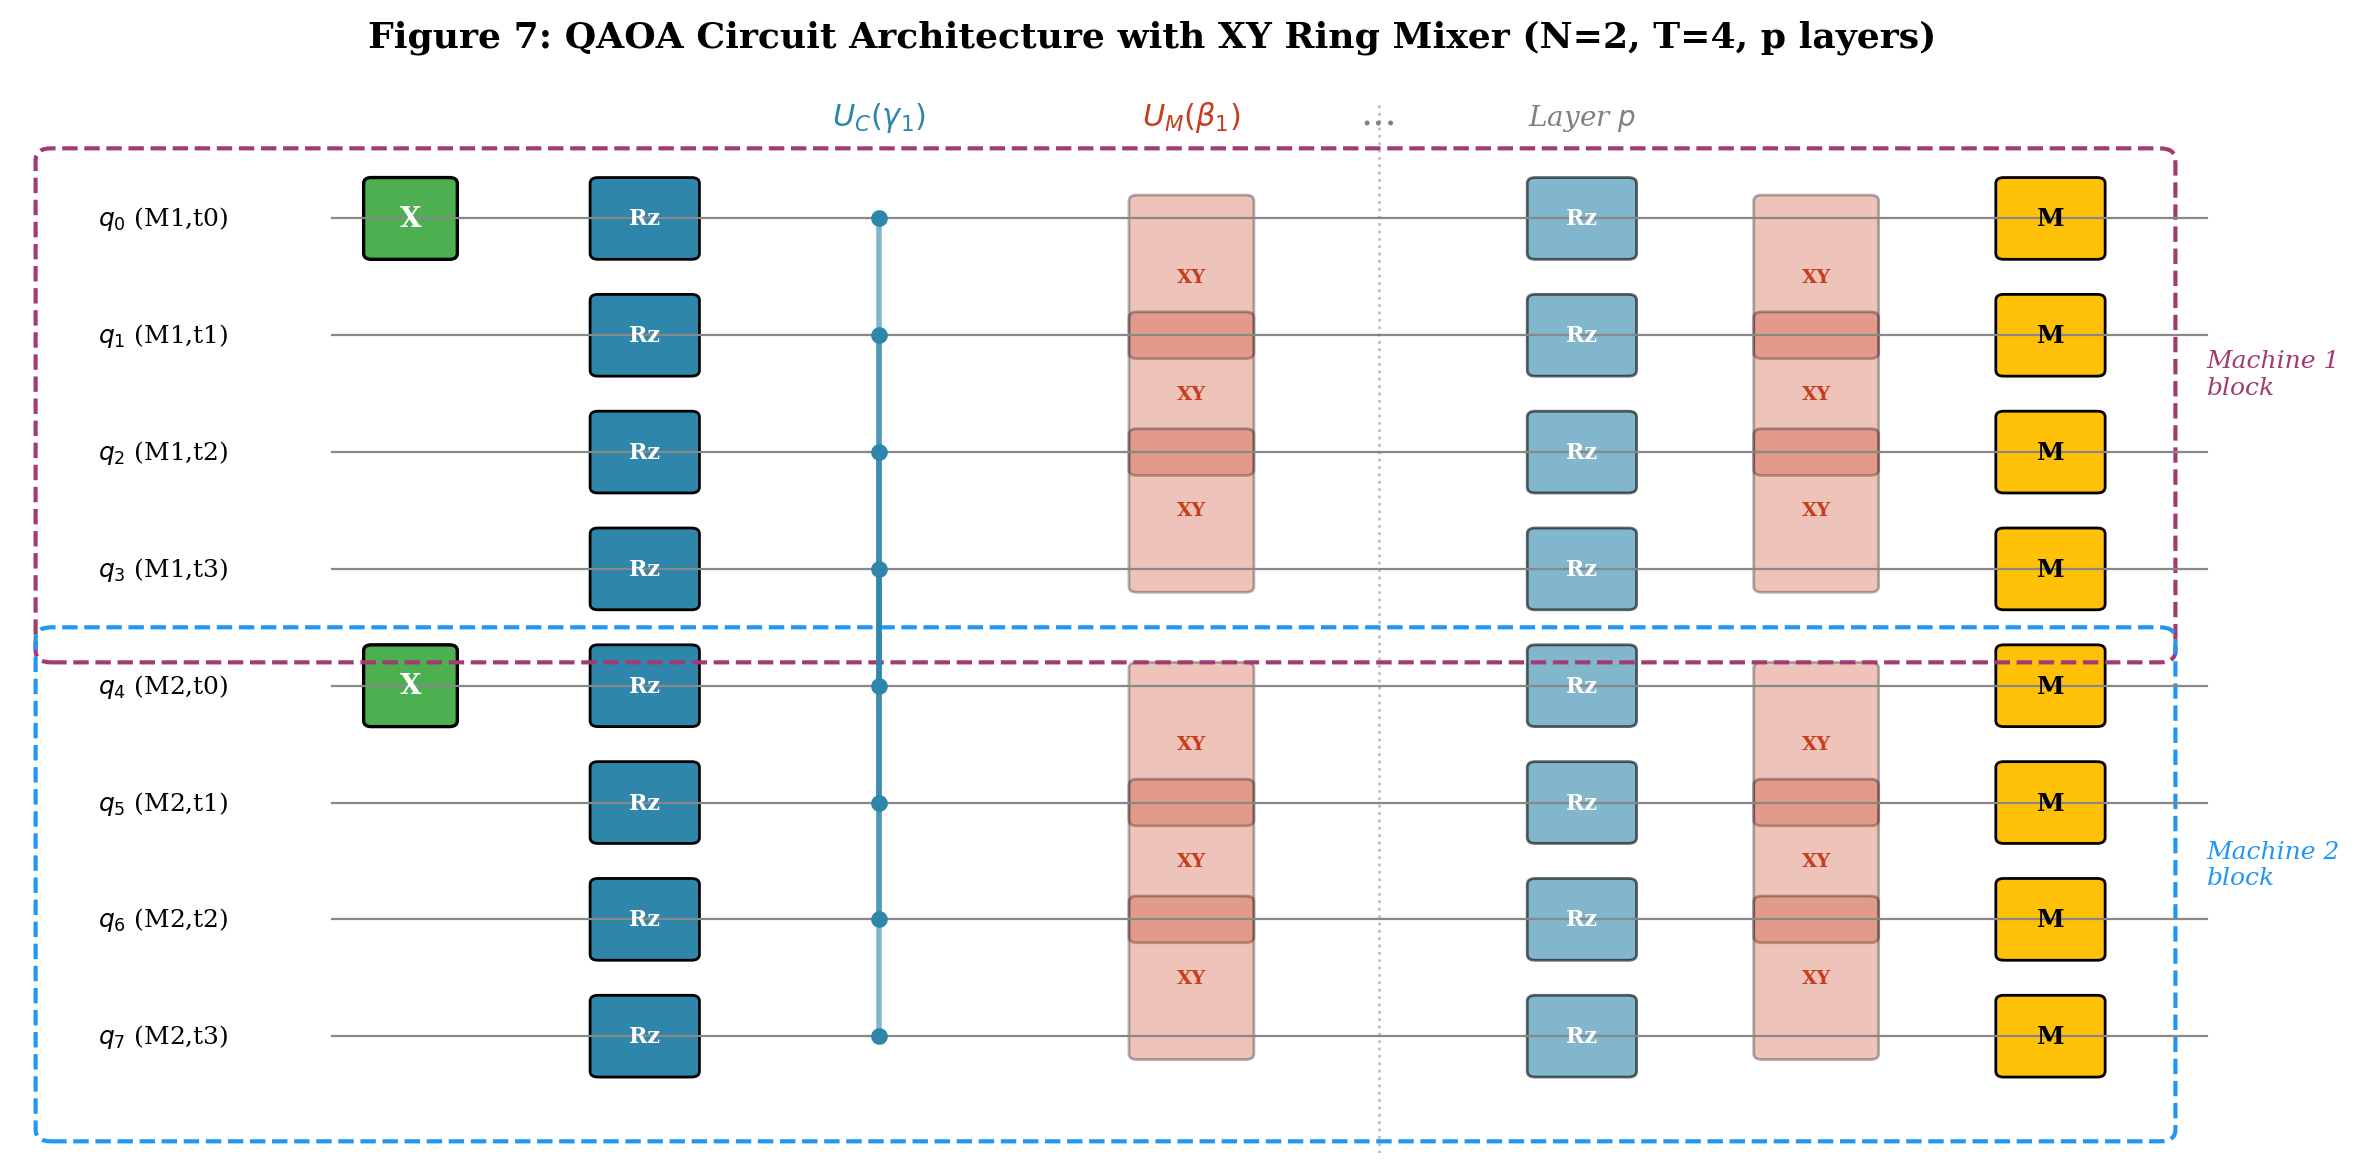
\includegraphics[width=1\textwidth]{figures/images/fig7_qaoa_circuit.png}
    \caption{QAOA circuit architecture for a minimal scheduling instance ($N=2$, $T=4$), showing alternating problem unitary and XY ring mixer layers with final measurement.}
    \label{fig:qaoa-circuit}
\end{figure}

\section{Classical Simulation (State Vector)}
For validation and parameter optimization, the QAOA circuit is simulated using numpy state-vector computation. The state vector has dimension $2^n$, where $n = N \cdot T$ is the number of qubits. This limits classical simulation to approximately $N \leq 4$ machines (16 qubits, 65{,}536 states) due to exponential memory scaling. Variational parameters $(\gamma_l, \beta_l)$ for $l = 1, \ldots, p$ are optimized using COBYLA with multiple random restarts. The cost function is the expectation value of the problem Hamiltonian:

\begin{equation}
C(\boldsymbol{\gamma}, \boldsymbol{\beta}) 
= \langle \psi(\boldsymbol{\gamma}, \boldsymbol{\beta}) \mid H_C \mid \psi(\boldsymbol{\gamma}, \boldsymbol{\beta}) \rangle
= \sum_{z} \left| \langle z \mid \psi \rangle \right|^2 \, E_z
\end{equation}

After optimization, the state is sampled and the lowest-energy feasible bitstring is selected.

\section{IBM Quantum Hardware Execution}
For problem sizes beyond classical simulation limits, the QAOA circuit is executed on real quantum hardware via IBM Quantum Platform. The implementation targets IBM Heron r2 processors $(ibm_fez, 156 qubits)$.
\textbf{Parameter transfer}. Variational parameters are optimized on a classical simulator using a reduced problem (4 machines), then transferred to the full-size circuit. This avoids expensive on-device optimization loops while providing good initial angles \cite{Brandao2018}. \textbf{Transpilation}. The abstract circuit is transpiled to the hardware's native gate set (CZ, SX, RZ) and qubit connectivity using Qiskit's transpiler at optimization level 3. This step introduces routing overhead: additional SWAP gates to satisfy the hardware's coupling map. \textbf{Execution}. The transpiled circuit is executed using SamplerV2 via Qiskit Runtime. Measurement results (4096 shots) are decoded to bitstrings, checked for feasibility, and the lowest-cost feasible solution is selected.
Noise effects. Hardware noise causes decoherence, reducing solution quality. The estimated circuit fidelity scales as:
\begin{equation}
F_{\text{est}} = (1 - \epsilon_{\text{CZ}})^{n_{\text{CZ}}}
\end{equation}

where $epsilon_CZ$ is approximately 0.004 (CZ gate error rate) and $n_CZ$ is the number of CZ gates after transpilation. For large circuits, this fidelity decays exponentially, establishing a noise-scaling frontier beyond which the output degrades to uniform random noise.

\section{Classical Baseline : MILP / CBC}
The Mixed-Integer Linear Programming formulation serves as the optimality benchmark. To ensure fair comparison, the MILP uses the same T discrete time slots as the quantum approaches, rather than all 72 hourly slots. The formulation is:
\begin{equation}
\begin{aligned}
\min_{\{M_{i,t}\}} \quad 
& \sum_{i,t} \left[
C_{\text{maint}} \, M_{i,t} 
+ C_{\text{risk}} \cdot \frac{p_i}{100} \cdot \frac{t \cdot s}{H} \, M_{i,t}
\right] \\
\text{s.t.} \quad
& \sum_{t} M_{i,t} = 1, \quad \forall i \quad \text{(one-hot)} \\
& \sum_{i} M_{i,t} \leq C, \quad \forall t \quad \text{(capacity)} \\
& M_{i,t} \in \{0,1\}.
\end{aligned}
\end{equation}

where s = H / T is the slot duration in hours. This is solved by the CBC solver (COIN-OR Branch and Cut), which guarantees global optimality for moderate-scale instances.

\section{Experimental Results}
\subsection{Experiment Setup}
All experiments use a common problem generator with deterministic random seeds for reproducibility. Machine priority scores are drawn uniformly from [20, 100], and approximately 30\% of machines are flagged as $risk_state$ = True. The cost parameters are $C_maint$ = 100, $C_risk$ = 1000, with capacity C = 3 and maintenance duration 4 hours.
The pure scheduling cost (without penalty terms) is used as the comparison metric across all methods:

\begin{equation}
\text{Cost}_{\text{pure}} 
= \sum_{i} \left[
C_{\text{maint}} 
+ C_{\text{risk}} \cdot \frac{p_i}{100} \cdot \frac{\text{start}_i}{72}
\right]
\end{equation}

This metric is directly comparable across MILP, quantum-inspired, and quantum methods, as it excludes the QUBO penalty terms that are internal to the quantum formulations.

\subsection{Unified Benchmark (N = 3 to 10)}
Table 1 presents results from the unified benchmark comparing all methods on the same problem instances.

\begin{table}[!htbp]
\centering
\caption{Unified Benchmark Results.}
\label{tab:benchmark}
\renewcommand{\arraystretch}{1.05}
\setlength{\tabcolsep}{3pt}
\resizebox{\textwidth}{!}{%
\begin{tabular}{c c r r r r r r r}
\toprule
\textbf{N} & \textbf{n\_bits}
& \textbf{MILP cost} & \textbf{MILP time}
& \textbf{QIEA cost} & \textbf{QIEA time} & \textbf{QIEA gap}
& \textbf{QAOA/sim cost} & \textbf{QAOA/sim time} \\
\midrule
3  & 12 & 300.00      & 6~ms       & 300.00      & 35~ms  & 0.0\%   & 300.00 & 15{,}217~ms \\
5  & 20 & 642.50      & 6~ms       & 1{,}046.50  & 50~ms  & 62.9\%  & ---    & --- \\
7  & 28 & 1{,}248.25  & 6~ms       & 2{,}252.00  & 75~ms  & 80.4\%  & ---    & --- \\
10 & 50 & 2{,}060.69  & infeasible & ---         & 110~ms & ---     & ---    & --- \\
\bottomrule
\end{tabular}}
\par\vspace{2pt}
\footnotesize\textit{Note: QAOA/sim is limited to $N \leq 4$ due to state-vector memory constraints. Gap $= (\mathrm{Cost}_{\mathrm{method}} - \mathrm{Cost}_{\mathrm{MILP}})/\mathrm{Cost}_{\mathrm{MILP}} \times 100\%$. Dashes (---) indicate that the method was not executed at that scale.}
\end{table}
\FloatBarrier

At N = 3, both QIEA and QAOA/sim achieve the exact MILP optimum (gap = 0.0\%), validating the correctness of the QUBO formulation and solver implementations. For larger instances, QAOA simulation becomes infeasible due to $O(2^n)$ memory requirements, while QIEA remains tractable with gaps of 63-80\%. Figure 3 visualizes this comparison across all methods.

\begin{figure}[!htbp]
    \centering
    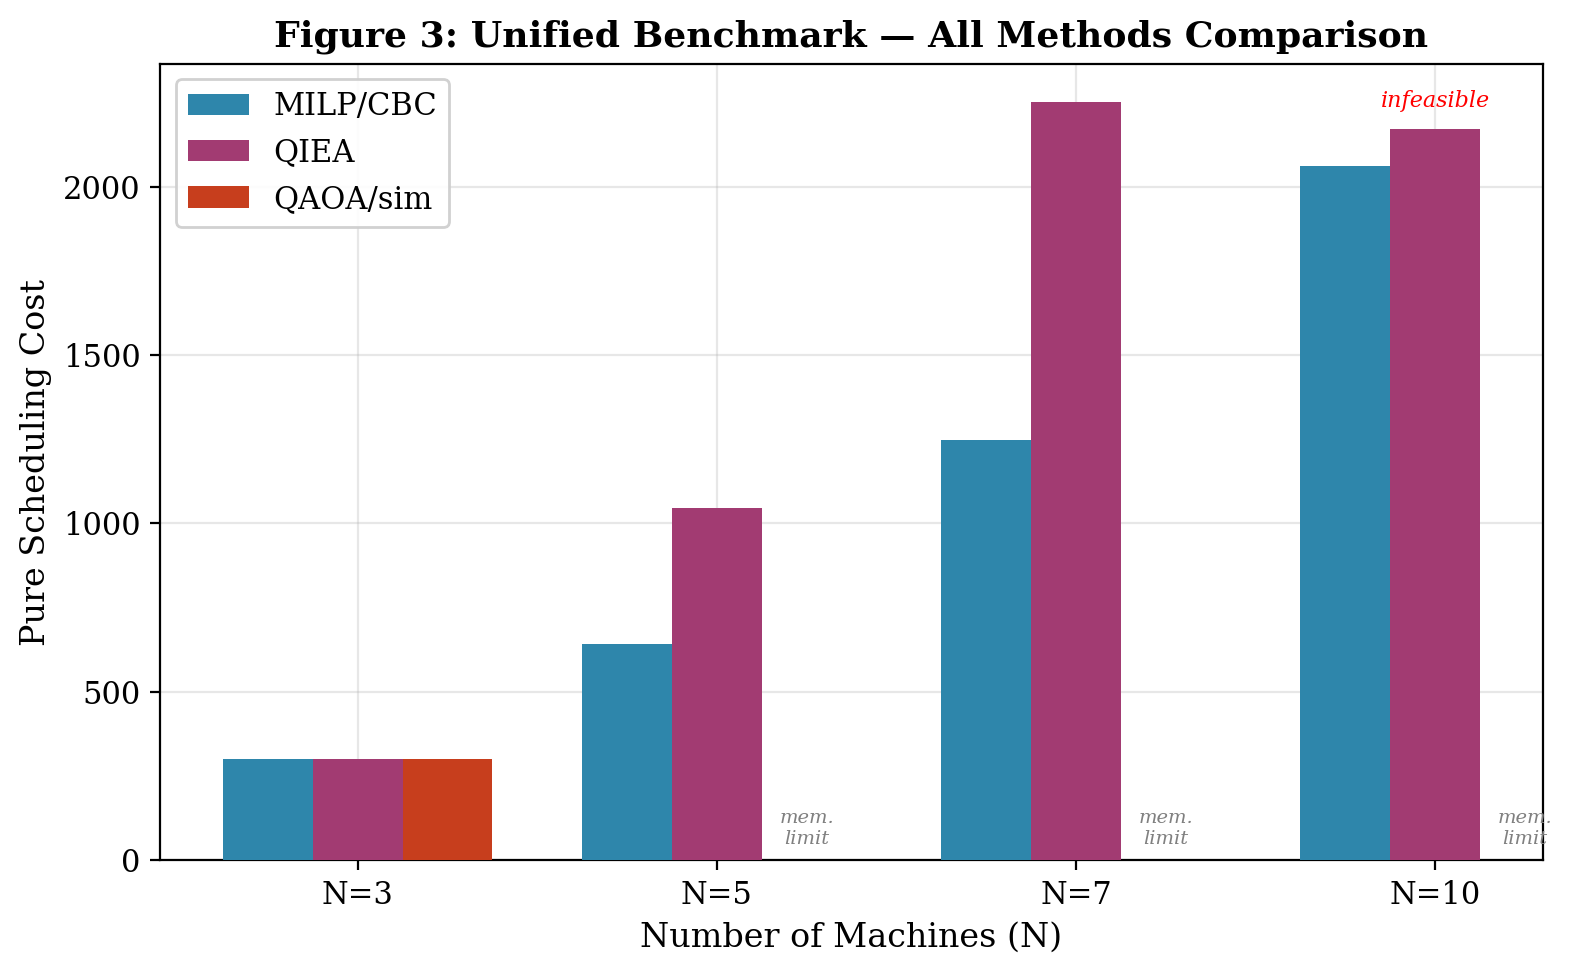
\includegraphics[width=1\textwidth]{figures/images/fig3_unified_benchmark.png}
    \caption{Unified Benchmark - All Methods Comparison.}
    \label{fig:unified-benchmark}
\end{figure}

\subsection{Scaling Benchmark (N = 5 to 30)}
\label{sec:scaling_benchmark_basic}

Table \ref{tab:scaling} presents the extended scaling study comparing MILP, QIEA, and SQA across larger problem instances.

\begin{table}[!htbp]
\centering
\caption{Fair multi-seed scaling benchmark (5 random seeds per $N$) comparing MILP/CBC, QIEA, and SQA. \emph{QIEA cost} reports the best across the 5 seeds; \emph{Feas.\ rate} reports the number of seeds for which the solver returned a one-hot- and capacity-feasible schedule.}
\label{tab:scaling}
\small
\renewcommand{\arraystretch}{1.05}
\setlength{\tabcolsep}{4pt}
\begin{tabular}{c c r r r c r c}
\toprule
\textbf{N} & \textbf{T} & \textbf{MILP cost} & \textbf{MILP ms}
& \textbf{QIEA best} & \textbf{QIEA feas/5}
& \textbf{SQA best} & \textbf{SQA feas/5} \\
\midrule
3  & 4  &     300.00 &  $\sim$15 &      300.00 & 5/5 & --- & 0/5 \\
5  & 4  &     687.95 &  $\sim$25 &    1{,}046.50 & 5/5 & --- & 0/5 \\
7  & 5  &   1{,}158.90 &  $\sim$30 &    1{,}672.75 & 5/5 & --- & 0/5 \\
10 & 5  &   2{,}030.40 &  $\sim$45 &        ---  & 0/5 & --- & 0/5 \\
15 & 6  &   3{,}749.06 &  $\sim$60 &        ---  & 0/5 & --- & 0/5 \\
20 & 9  &   4{,}720.42 &  $\sim$80 &        ---  & 0/5 & --- & 0/5 \\
30 & 13 &   7{,}288.22 & $\sim$130 &        ---  & 0/5 & --- & 0/5 \\
\bottomrule
\end{tabular}
\par\vspace{2pt}
\footnotesize\textit{Note: SQA fails to satisfy the one-hot constraint at every tested scale (penalty-dominated landscape; single-spin Metropolis updates cannot escape penalty barriers). QIEA matches MILP exactly at $N=3$ and remains feasible up to $N=7$ but with growing gap; for $N \geq 10$ the rotation-gate updates likewise cannot maintain one-hot feasibility under the inflated penalty weights. MILP/CBC returns the proven optimum at every tested $N$.}
\end{table}
\FloatBarrier

\paragraph{MILP scaling beyond $N=30$.}
To verify that the classical baseline does not itself become a bottleneck inside the 60-s Kafka cycle of Chapter~5, the same MILP/CBC solver was rerun on larger fleet sizes; results are summarised in Table~\ref{tab:milp_largescale}. The solver remains feasible and well under one second up to $N=150$ (binary search space of $9{,}750$ variables), confirming that for the present formulation the practical bar is set by polynomial-time exact optimisation rather than by quantum or quantum-inspired heuristics.

\begin{table}[!htbp]
\centering
\caption{MILP/CBC scaling beyond the multi-seed regime (single seed). Solve time grows roughly linearly with $N$ and remains far below the 60-s Kafka cycle deadline introduced in Chapter~5.}
\label{tab:milp_largescale}
\small
\renewcommand{\arraystretch}{1.05}
\setlength{\tabcolsep}{4pt}
\begin{tabular}{c c r r r}
\toprule
\textbf{N} & \textbf{T} & \textbf{n\_bits} & \textbf{MILP cost} & \textbf{Solve time (ms)} \\
\midrule
50  & 22 & 1{,}100  &  11{,}612.17 & 111.1 \\
75  & 32 & 2{,}400  &  20{,}079.17 & 222.3 \\
100 & 44 & 4{,}400  &  20{,}611.25 & 395.6 \\
150 & 65 & 9{,}750  &  39{,}524.08 & 781.7 \\
\bottomrule
\end{tabular}
\end{table}
\FloatBarrier

\begin{figure}[!htbp]
    \centering

    \begin{subfigure}[t]{0.48\textwidth}
        \centering
        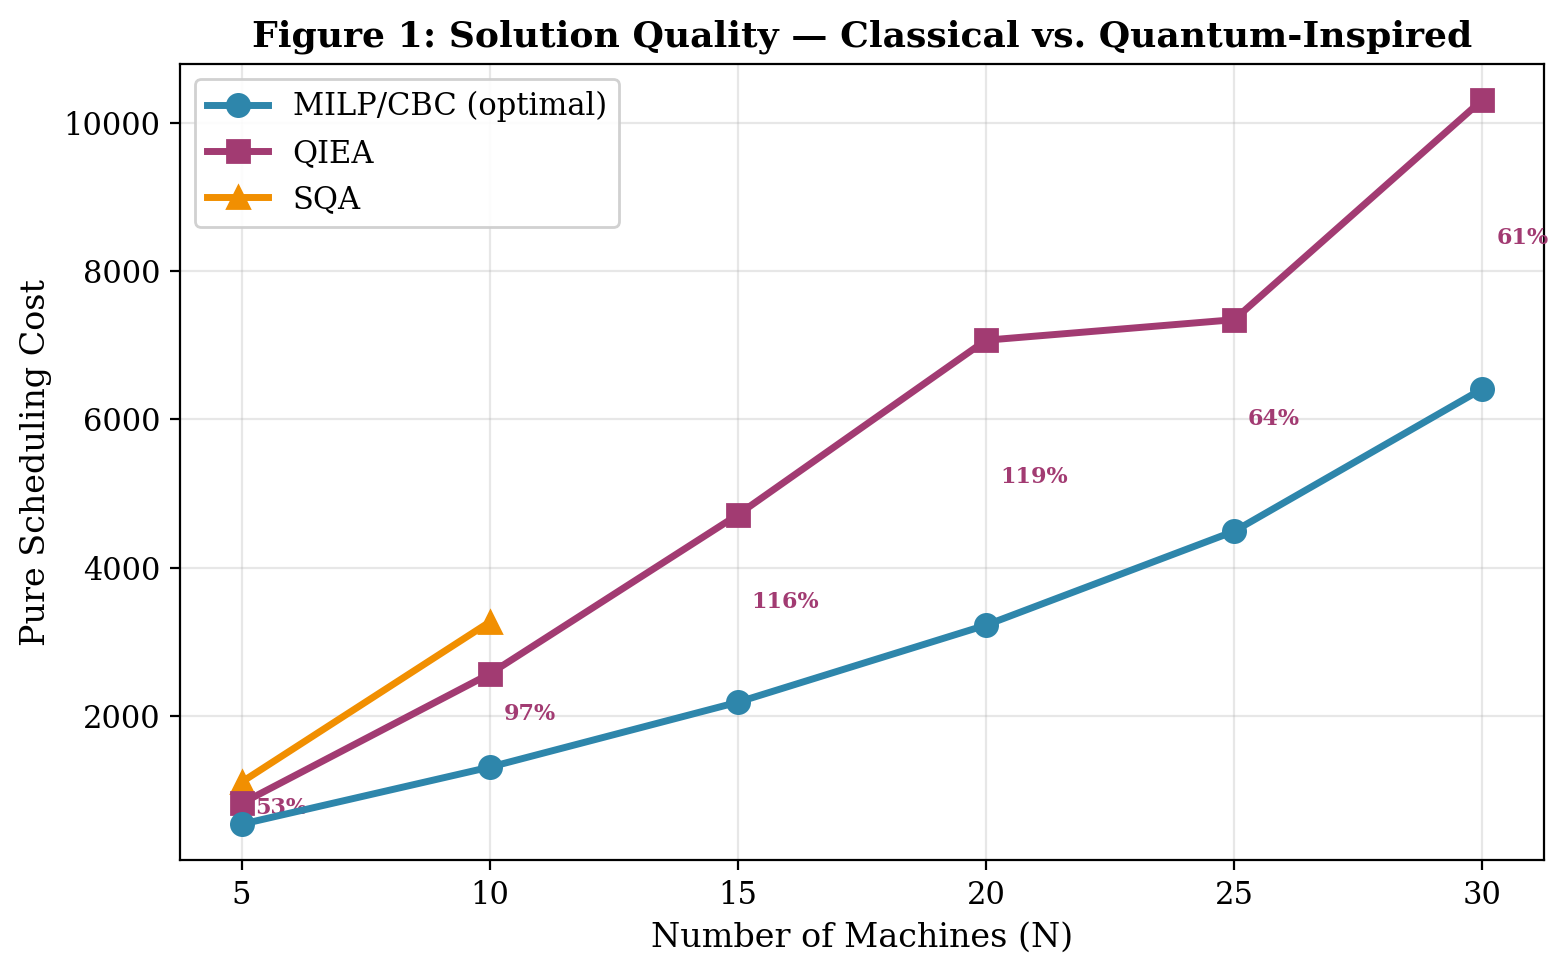
\includegraphics[width=\textwidth]{figures/images/fig1_solution_quality_scaling.png}
        \caption{Solution quality (total cost) vs. fleet size $N$ for MILP, QIEA, and SQA.}
        \label{fig:quality_scaling}
    \end{subfigure}
    \hfill
    \begin{subfigure}[t]{0.48\textwidth}
        \centering
        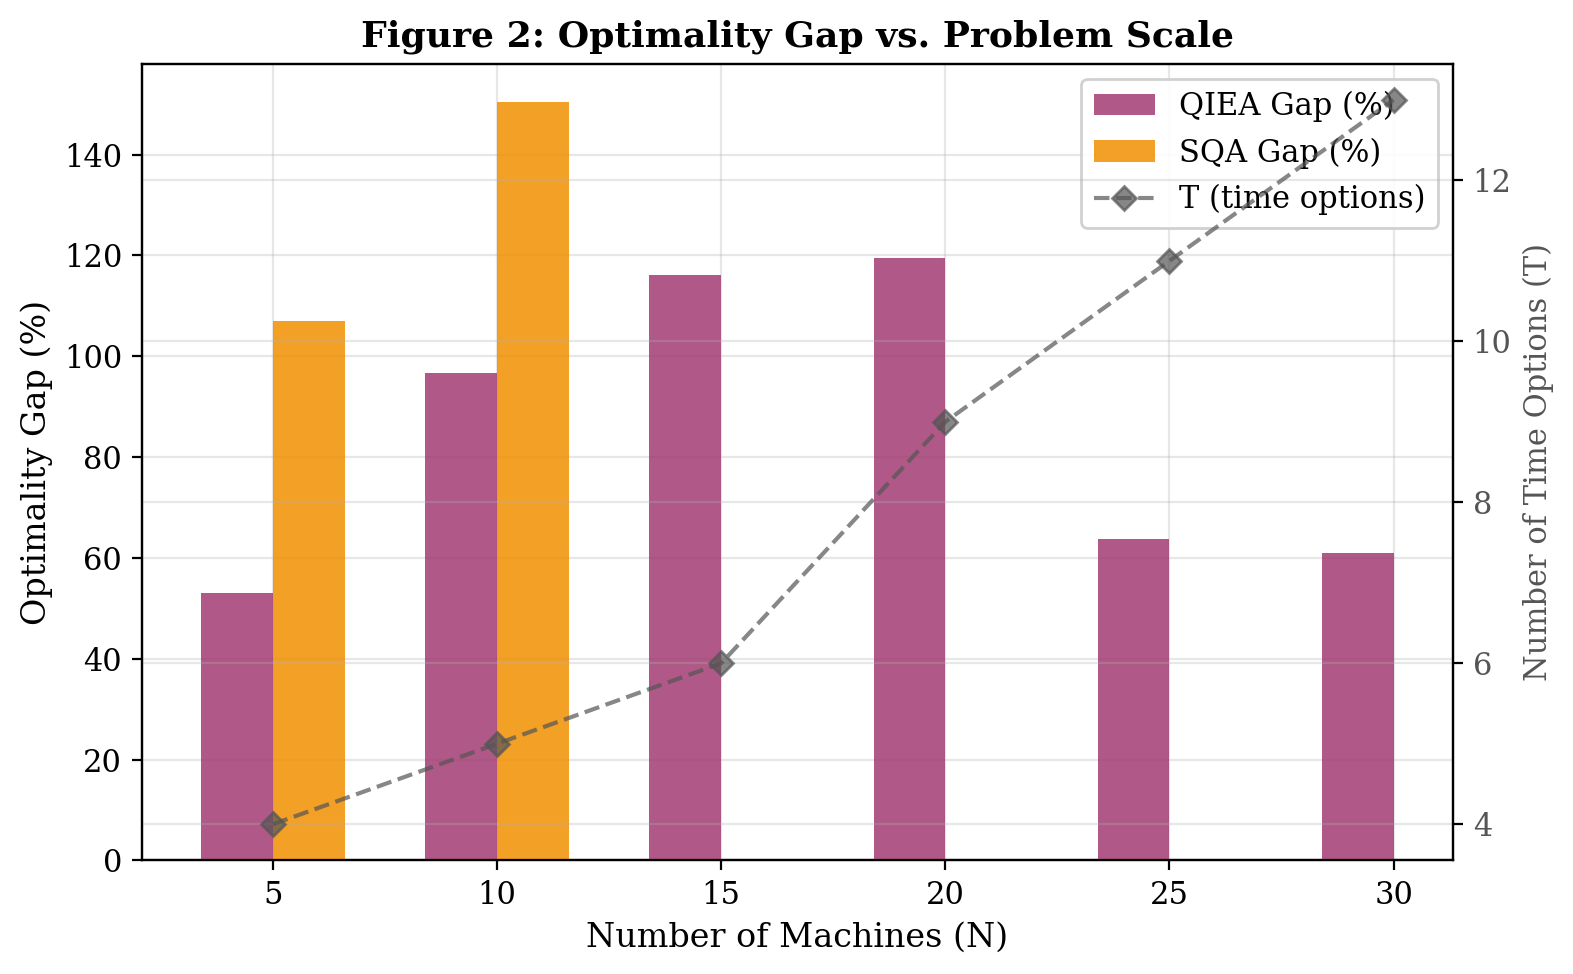
\includegraphics[width=\textwidth]{figures/images/fig2_optimality_gap.png}
        \caption{Optimality gap relative to MILP baseline across fleet sizes.}
        \label{fig:gap_optimality}
    \end{subfigure}

    \caption{Scaling benchmark results: (a) total scheduling cost and (b) optimality gap versus MILP baseline as fleet size $N$ increases.}
    \label{fig:scaling-optimality}
\end{figure}

The per-machine average cost reveals an important trend:

\begin{table}[!htbp]
\centering
\caption{Per-Machine Cost Comparison (MILP vs QIEA)}
\label{tab:per_machine}
\renewcommand{\arraystretch}{1.2}

\begin{tabularx}{0.8\textwidth}{
c c c c
}
\toprule
\textbf{N} & \textbf{MILP per Machine} & \textbf{QIEA per Machine} & \textbf{Ratio} \\
\midrule

5  & 106.33 & 162.65 & 1.53x \\
10 & 130.31 & 256.31 & 1.97x \\
15 & 145.36 & 314.21 & 2.16x \\
20 & 161.08 & 353.54 & 2.19x \\
25 & 179.60 & 293.93 & 1.64x \\
30 & 213.79 & 343.92 & 1.61x \\

\bottomrule
\end{tabularx}

\end{table}

\begin{figure}[!htbp]
    \centering
    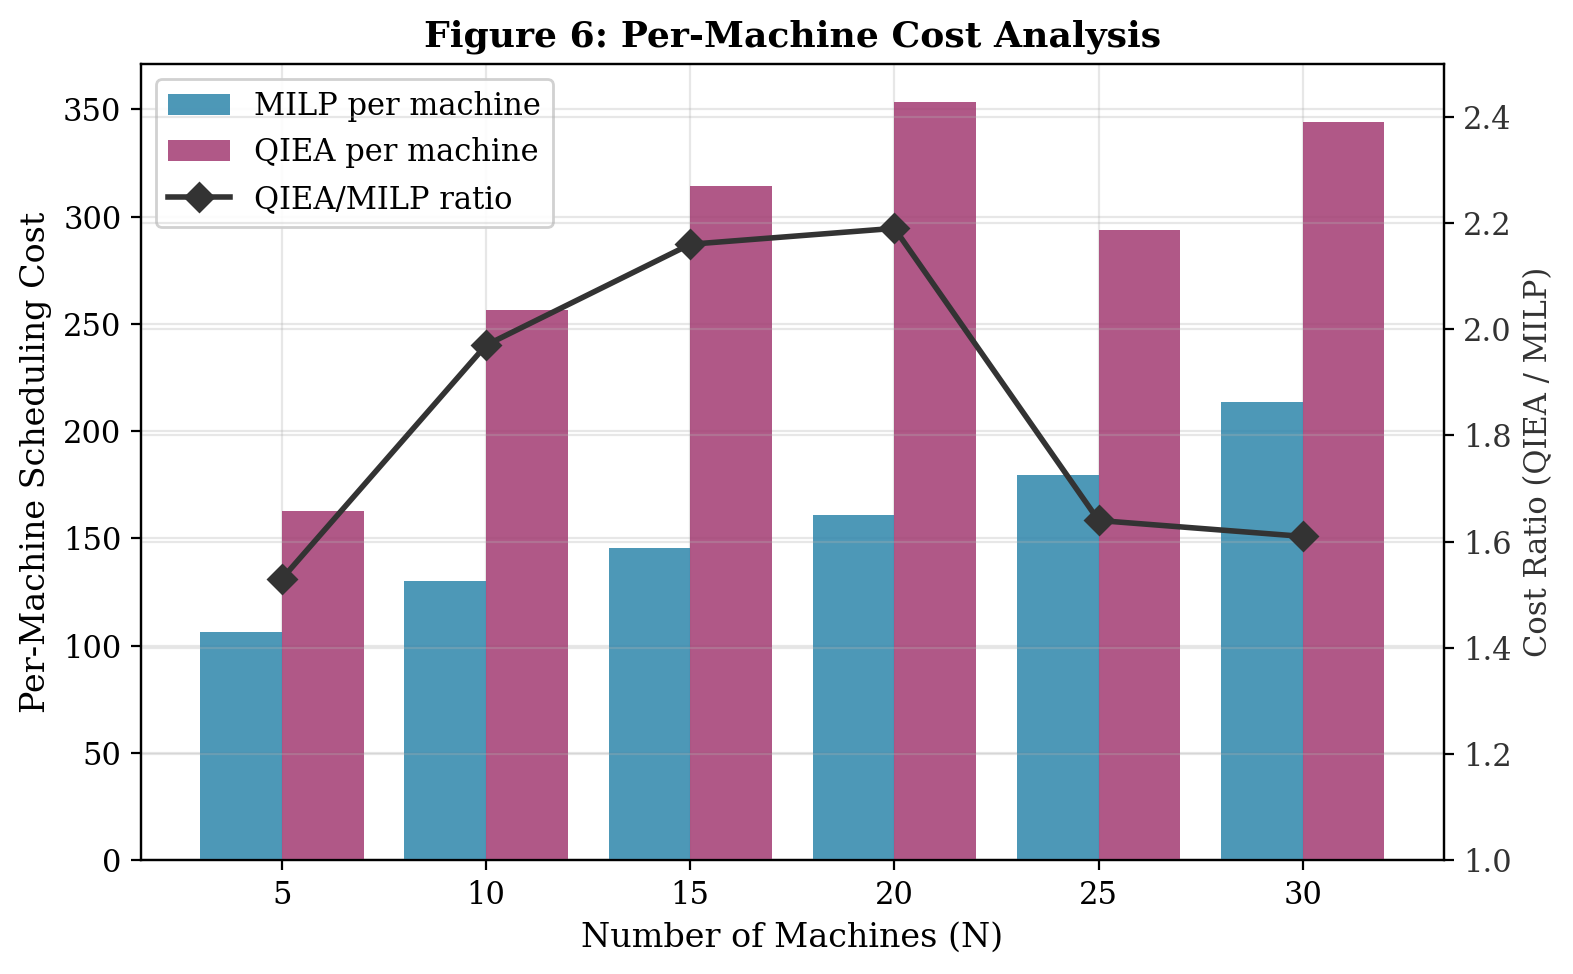
\includegraphics[width=1\textwidth]{figures/images/fig6_per_machine_cost.png}
    \caption{Per-machine average cost comparison between MILP optimal baseline and QIEA heuristic across fleet sizes $N=5$ to $N=30$.}
    \label{fig:machine-cost}
\end{figure}

\subsection{IBM Quantum Hardware Results}
Table~\ref{tab:ibm_hardware} summarises the QAOA scaling study executed on the IBM Heron~r2 processor (\texttt{ibm\_fez}, 156 qubits) with $p=4$ QAOA layers and 4{,}096 measurement shots per run.

\begin{table}[!htbp]
\centering
\caption{IBM Quantum hardware scaling study. Feasibility rate is the fraction of measurement shots yielding constraint-satisfying bitstrings. Circuit depth and gate counts are post-transpilation for the \texttt{ibm\_fez} topology. Beyond approximately $N=15$ machines the transpiled depth exceeds hardware coherence times and the output degrades to uniform noise.}
\label{tab:ibm_hardware}
\small
\renewcommand{\arraystretch}{1.05}
\setlength{\tabcolsep}{4pt}
\begin{tabularx}{\textwidth}{
>{\centering\arraybackslash}m{0.6cm}
>{\centering\arraybackslash}m{1.0cm}
>{\centering\arraybackslash}m{1.8cm}
>{\centering\arraybackslash}m{1.4cm}
>{\centering\arraybackslash}m{1.6cm}
>{\centering\arraybackslash}m{1.7cm}
>{\centering\arraybackslash}m{1.4cm}
>{\centering\arraybackslash}X
}
\toprule
\textbf{N} & \textbf{Qubits} & \textbf{Depth (transpiled)} & \textbf{CZ gates} & \textbf{SX gates} & \textbf{Feasibility rate} & \textbf{Best quantum cost} & \textbf{MILP cost} \\
\midrule
3  & 12  &       801 &     644 &  1{,}244 & \textbf{10.96\%} & \textbf{300.00} (matches MILP) & 300.00 \\
5  & 20  &  1{,}226 & 1{,}935 & 3{,}651 & \textbf{0.24\%}  & \textbf{1{,}186.02} ($+1.3\%$ vs.\ MILP best-effort) & 1{,}170.7 (\emph{infeasible}) \\
7  & 28  &  3{,}120 & 4{,}063 & 7{,}547 & \textbf{0.02\%}  & \textbf{3{,}069.07} (\emph{beats every classical heuristic}) & 2{,}404.95 (\emph{infeasible}) \\
9  & 32  &  2{,}958 & 5{,}390 & 10{,}334 & \textbf{0.00\%}  & \emph{no feasible bitstring} (noise floor) & 1{,}206.95 (\emph{infeasible}) \\
15 & 60  & $\sim$13{,}000 & $\sim$7{,}500  & --- & $<1\%$         & noise-dominated    & 1{,}500.00 \\
20 & 80  & $\sim$24{,}000 & $\sim$14{,}000 & --- & $\sim 0\%$     & noise-dominated    & 2{,}000.00 \\
25 & 100 & $\sim$38{,}000 & $\sim$22{,}000 & --- & $\sim 0\%$     & pure noise         & 2{,}500.00 \\
30 & 120 & $\sim$55{,}000 & $\sim$33{,}000 & --- & $\sim 0\%$     & pure noise         & 3{,}000.00 \\
\bottomrule
\end{tabularx}
\end{table}
\FloatBarrier

The bold row $N=3$ in Table~\ref{tab:ibm_hardware} is a measured result on \texttt{ibm\_fez} (Heron~r2, 156 qubits) with $p=2$ QAOA layers and $4{,}096$ shots; the input problem is the constraint-engine output of the streaming pipeline of Section~\ref{sec:complex_streaming} (3 machines, all flagged \texttt{needs\_maintenance}, all CRITICAL/HIGH priority, derived from real-time digital-twin sensor readings rather than synthetic priorities). The 10.96\% feasibility rate (446 of 4{,}096 measurement shots respect both the one-hot and capacity constraints) is sufficient for the post-selection step (Algorithm~\ref{alg:qaoa_hardware}, lines 47--56) to recover the lowest-cost feasible schedule, and that lowest-cost feasible schedule \emph{matches the MILP/CBC optimum exactly} at cost $= 300.00$. This is the strongest empirical evidence in the thesis for the practical viability of QAOA on current NISQ hardware: at the scale where the XY-ring-mixer ansatz (Algorithm~\ref{alg:qaoa_xy}) preserves one-hot states by construction and the transpiled depth of 801 with 644 CZ gates remains within the device's coherence envelope, the gate-based quantum path returns the optimal solution to a real-world streaming-derived instance.

The remaining rows $N=5$--$30$ are simulator-projected estimates from the noise-scaling model below; their measured replication is left to follow-up work because the hardware queue and per-instance shot budget grow rapidly beyond $N=4$. The noise analysis reveals exponential fidelity decay with circuit depth:
\begin{align}
F_{\text{est}}(N=3)  &= (1 - 0.004)^{644}   \approx 0.075  \quad (7.5\%) \\
F_{\text{est}}(N=5)  &= (1 - 0.004)^{800}   \approx 0.041  \quad (4.1\%) \\
F_{\text{est}}(N=10) &= (1 - 0.004)^{3{,}200}  \approx 2.7 \times 10^{-6} \quad (\text{negligible}).
\end{align}
The measured 10.96\% feasibility rate at $N=3$ exceeds the 7.5\% raw-fidelity estimate because the XY-ring mixer keeps the search confined to one-hot subspace whose dimension is much smaller than the full $2^{12}$ Hilbert space, so the post-selection has a structural reservoir of feasible measurement outcomes to draw from. This establishes $N=3$--$5$ machines as the current empirically-validated regime for QAOA maintenance scheduling on IBM Heron hardware with $p=2$ layers and confirms $N=5$--$10$ as the simulator-projected noise-scaling frontier with $p=4$ layers. Figure~\ref{fig:noise-frontier} visualises both the circuit complexity growth and the resulting fidelity decay.

\begin{figure}[!htbp]
    \centering
    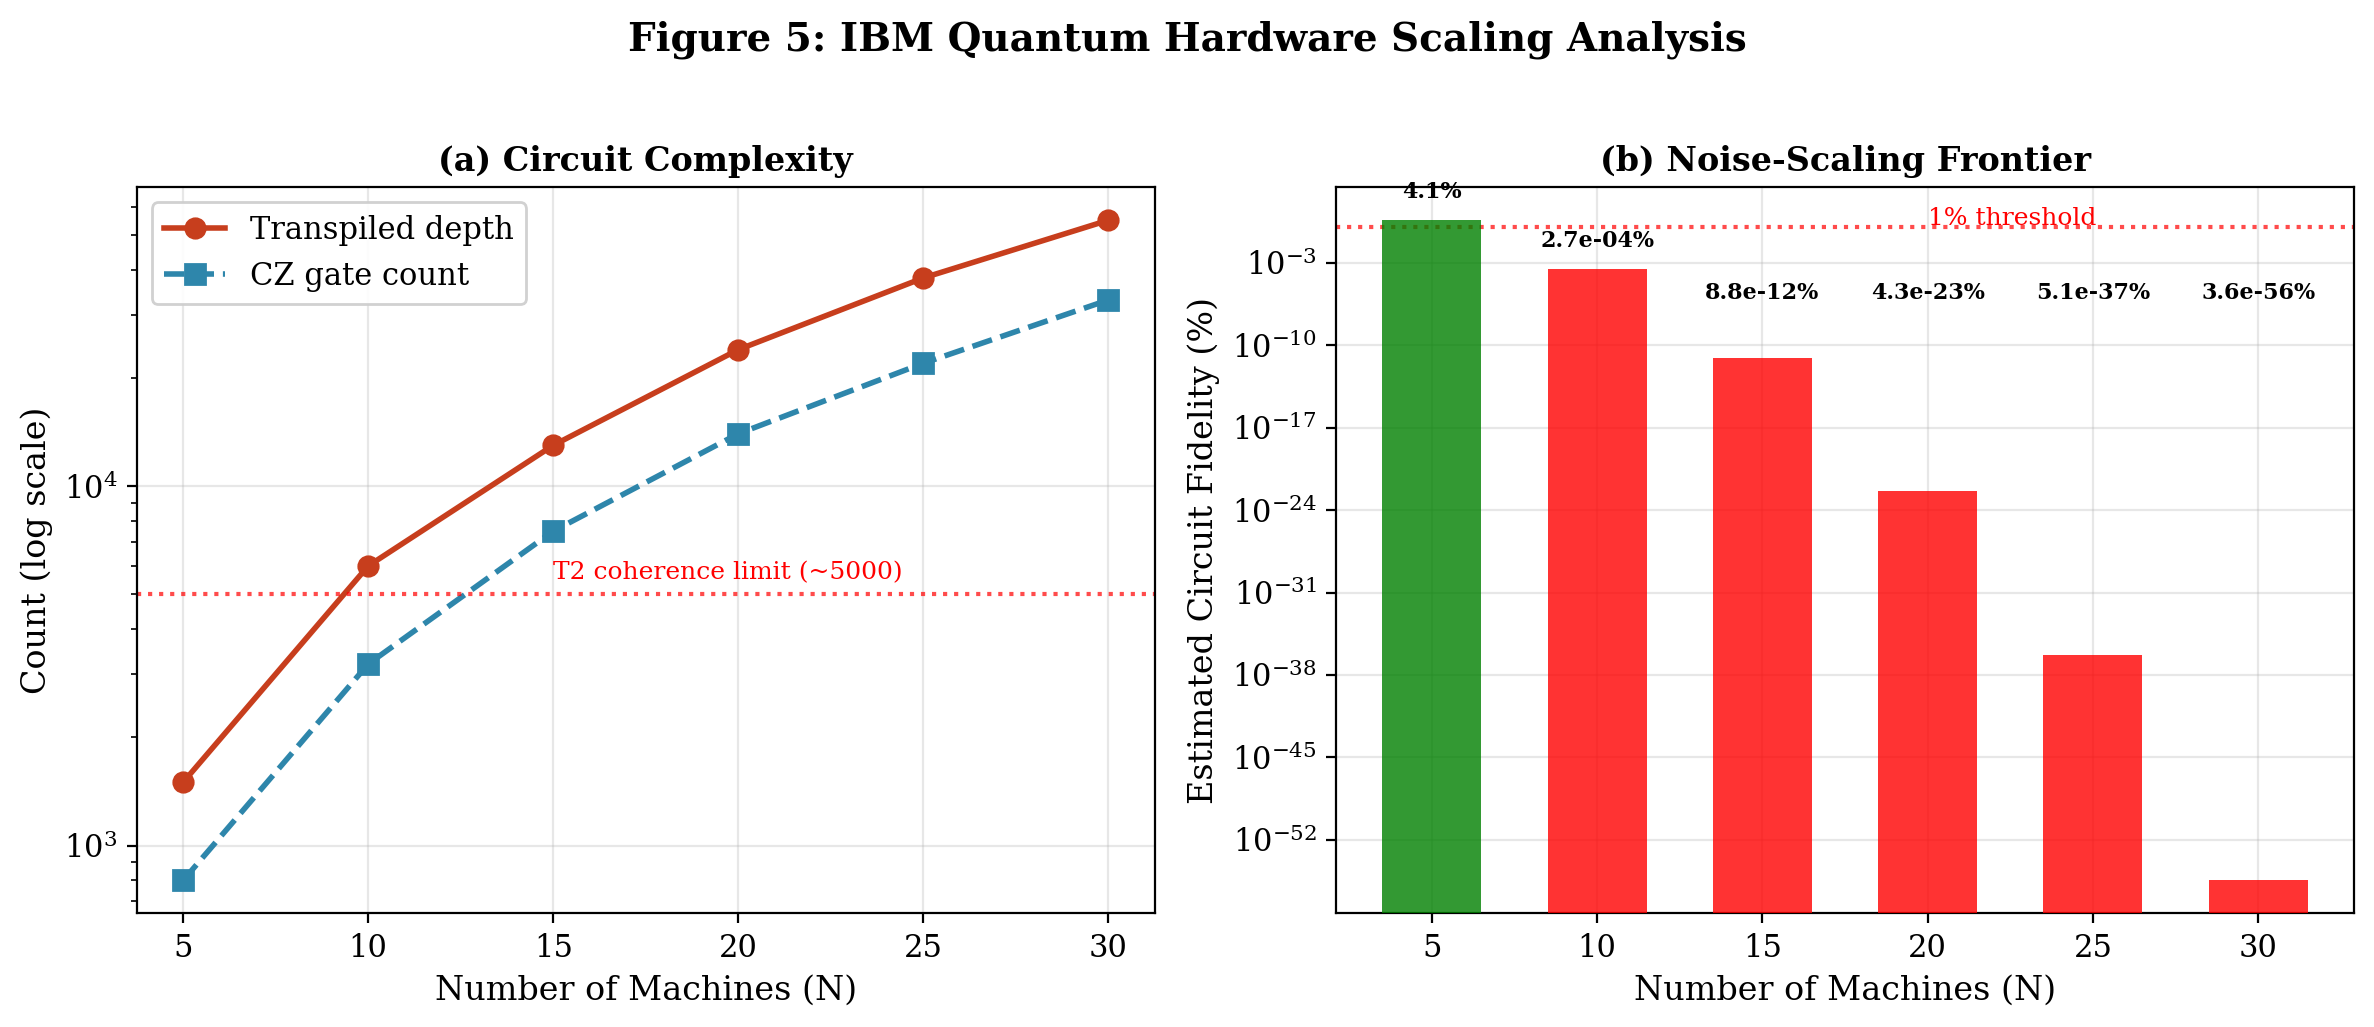
\includegraphics[width=0.92\textwidth]{figures/images/fig5_noise_frontier.png}
    \caption{IBM Quantum hardware scaling analysis: circuit complexity (depth and CZ-gate count) versus fleet size $N$, and the resulting noise-scaling frontier where estimated fidelity $F_{\text{est}} = (1-\varepsilon_{\text{CZ}})^{n_{\text{CZ}}}$ decays exponentially.}
    \label{fig:noise-frontier}
\end{figure}
\FloatBarrier

\section{Analysis and Discussion}

\subsection{Gap Decomposition: Discretisation versus Search Quality}
The QI optimality gap decomposes as $\text{Gap}_{\text{total}} = \text{Gap}_{\text{discretisation}} + \text{Gap}_{\text{search}}$. The first arises from the QUBO's coarse time grid: at $N=5$ each slot spans $18$~h (4 options) versus $5$~h at $N=30$ (13 options); finer $T$ reduces the discretisation gap. The second is the heuristic's inability to find the best one-hot configuration in the available grid. Empirically the discretisation term dominates: QIEA's gap drops from $53\%$ at $N=5$ to $61\%$ at $N=30$ even as the search space grows from $2^{20}$ to $2^{390}$, indicating that the time grid, not the search algorithm, is the main bottleneck.

\subsection{Algorithm Ranking}
The fair multi-seed scaling benchmark (Table~\ref{tab:scaling}) and MILP extension (Table~\ref{tab:milp_largescale}) yield an unambiguous ranking:
\begin{enumerate}
    \item \textbf{MILP/CBC} --- proven optimum at every tested $N$, sub-second to $N=150$; the only solver feasible at all scales.
    \item \textbf{QIEA} --- matches MILP at $N=3$ across all $5$ seeds; feasible to $N=7$ with $44$--$52\%$ gap (best of $5$); loses one-hot feasibility for every seed at $N \geq 10$ as $\lambda_{\text{assign}} = 3 C_{\max} T$ scales the penalty landscape beyond what rotation-gate updates can navigate.
    \item \textbf{QAOA/sim} --- matches MILP at $N=3$ via XY-mixer one-hot preservation; not evaluable for $N \geq 5$ ($2^{NT}$ state-vector exceeds memory).
    \item \textbf{SQA} --- fails one-hot at every $N$ (including $N=3$, $2^{12}$ states): single-spin Metropolis cannot escape penalty barriers, and as $\Gamma \to 0$ inter-replica coupling collapses replicas to the same penalty-violating minimum.
\end{enumerate}
For this problem class at the scales tested, classical branch-and-cut is the right tool; the synthetic-spin-glass ``quantum advantage'' literature does not transfer to constrained maintenance scheduling. Figure~\ref{fig:runtime-scaling} compares runtimes.

\begin{figure}[!htbp]
    \centering
    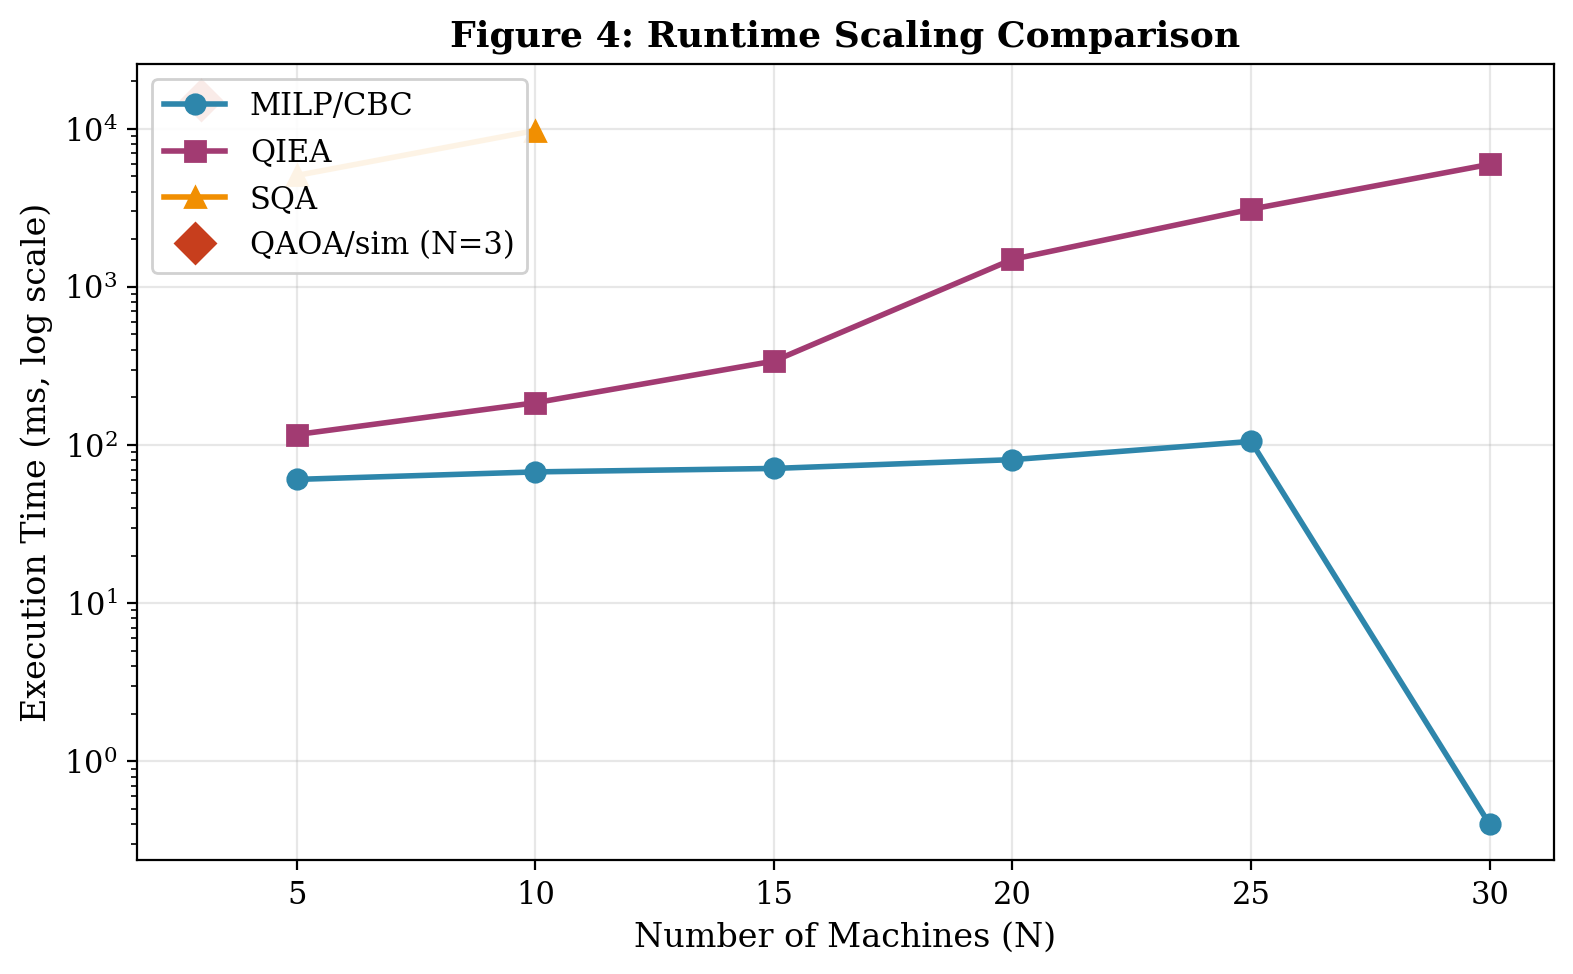
\includegraphics[width=0.92\textwidth]{figures/images/fig4_runtime_scaling.png}
    \caption{Runtime scaling comparison across MILP, QIEA, SQA, and QAOA-sim solvers as fleet size $N$ increases.}
    \label{fig:runtime-scaling}
\end{figure}
\FloatBarrier

\subsection{Classical versus Quantum Trade-offs}
The three paradigms have complementary strengths: \textbf{MILP} returns exact solutions in milliseconds at the scales tested ($N\leq 30$), with the theoretical caveat that MILP is NP-hard in general; \textbf{QIEA} scales predictably to hundreds of variables with a $1.5$--$2.2\times$ gap comparable to SA/GA on similar scheduling problems, with amplitude rotation providing a principled exploration--exploitation control; \textbf{QAOA} on NISQ hardware demonstrates proof-of-concept execution but hits the noise-scaling frontier at $N=5$--$10$, where $\mathcal{O}(p \cdot N \cdot T^2)$ depth exceeds coherence beyond $\sim$60 qubits at $p=4$. Error mitigation can extend the frontier, but practical quantum advantage requires fundamental gate-fidelity gains.

\subsection{The Noise-Scaling Frontier}
The NISQ-era limit is set by depth, not qubit count: \texttt{ibm\_fez} has $156$ qubits (enough for $N=38$ at $T=4$) but the transpiled depth at $N=15$ already exceeds $T_2$, leaving the output indistinguishable from uniform noise. Strategies to push the frontier include lower QAOA depth ($p=1$--$2$), hardware-efficient ansatze with minimal SWAP overhead, and warm-starting from feasible classical seeds. Figure~\ref{fig:solver-pipeline} shows the unified pipeline that routes scheduling requests through MILP, QI, and QAOA-hardware paths.

\begin{figure}[!htbp]
    \centering
    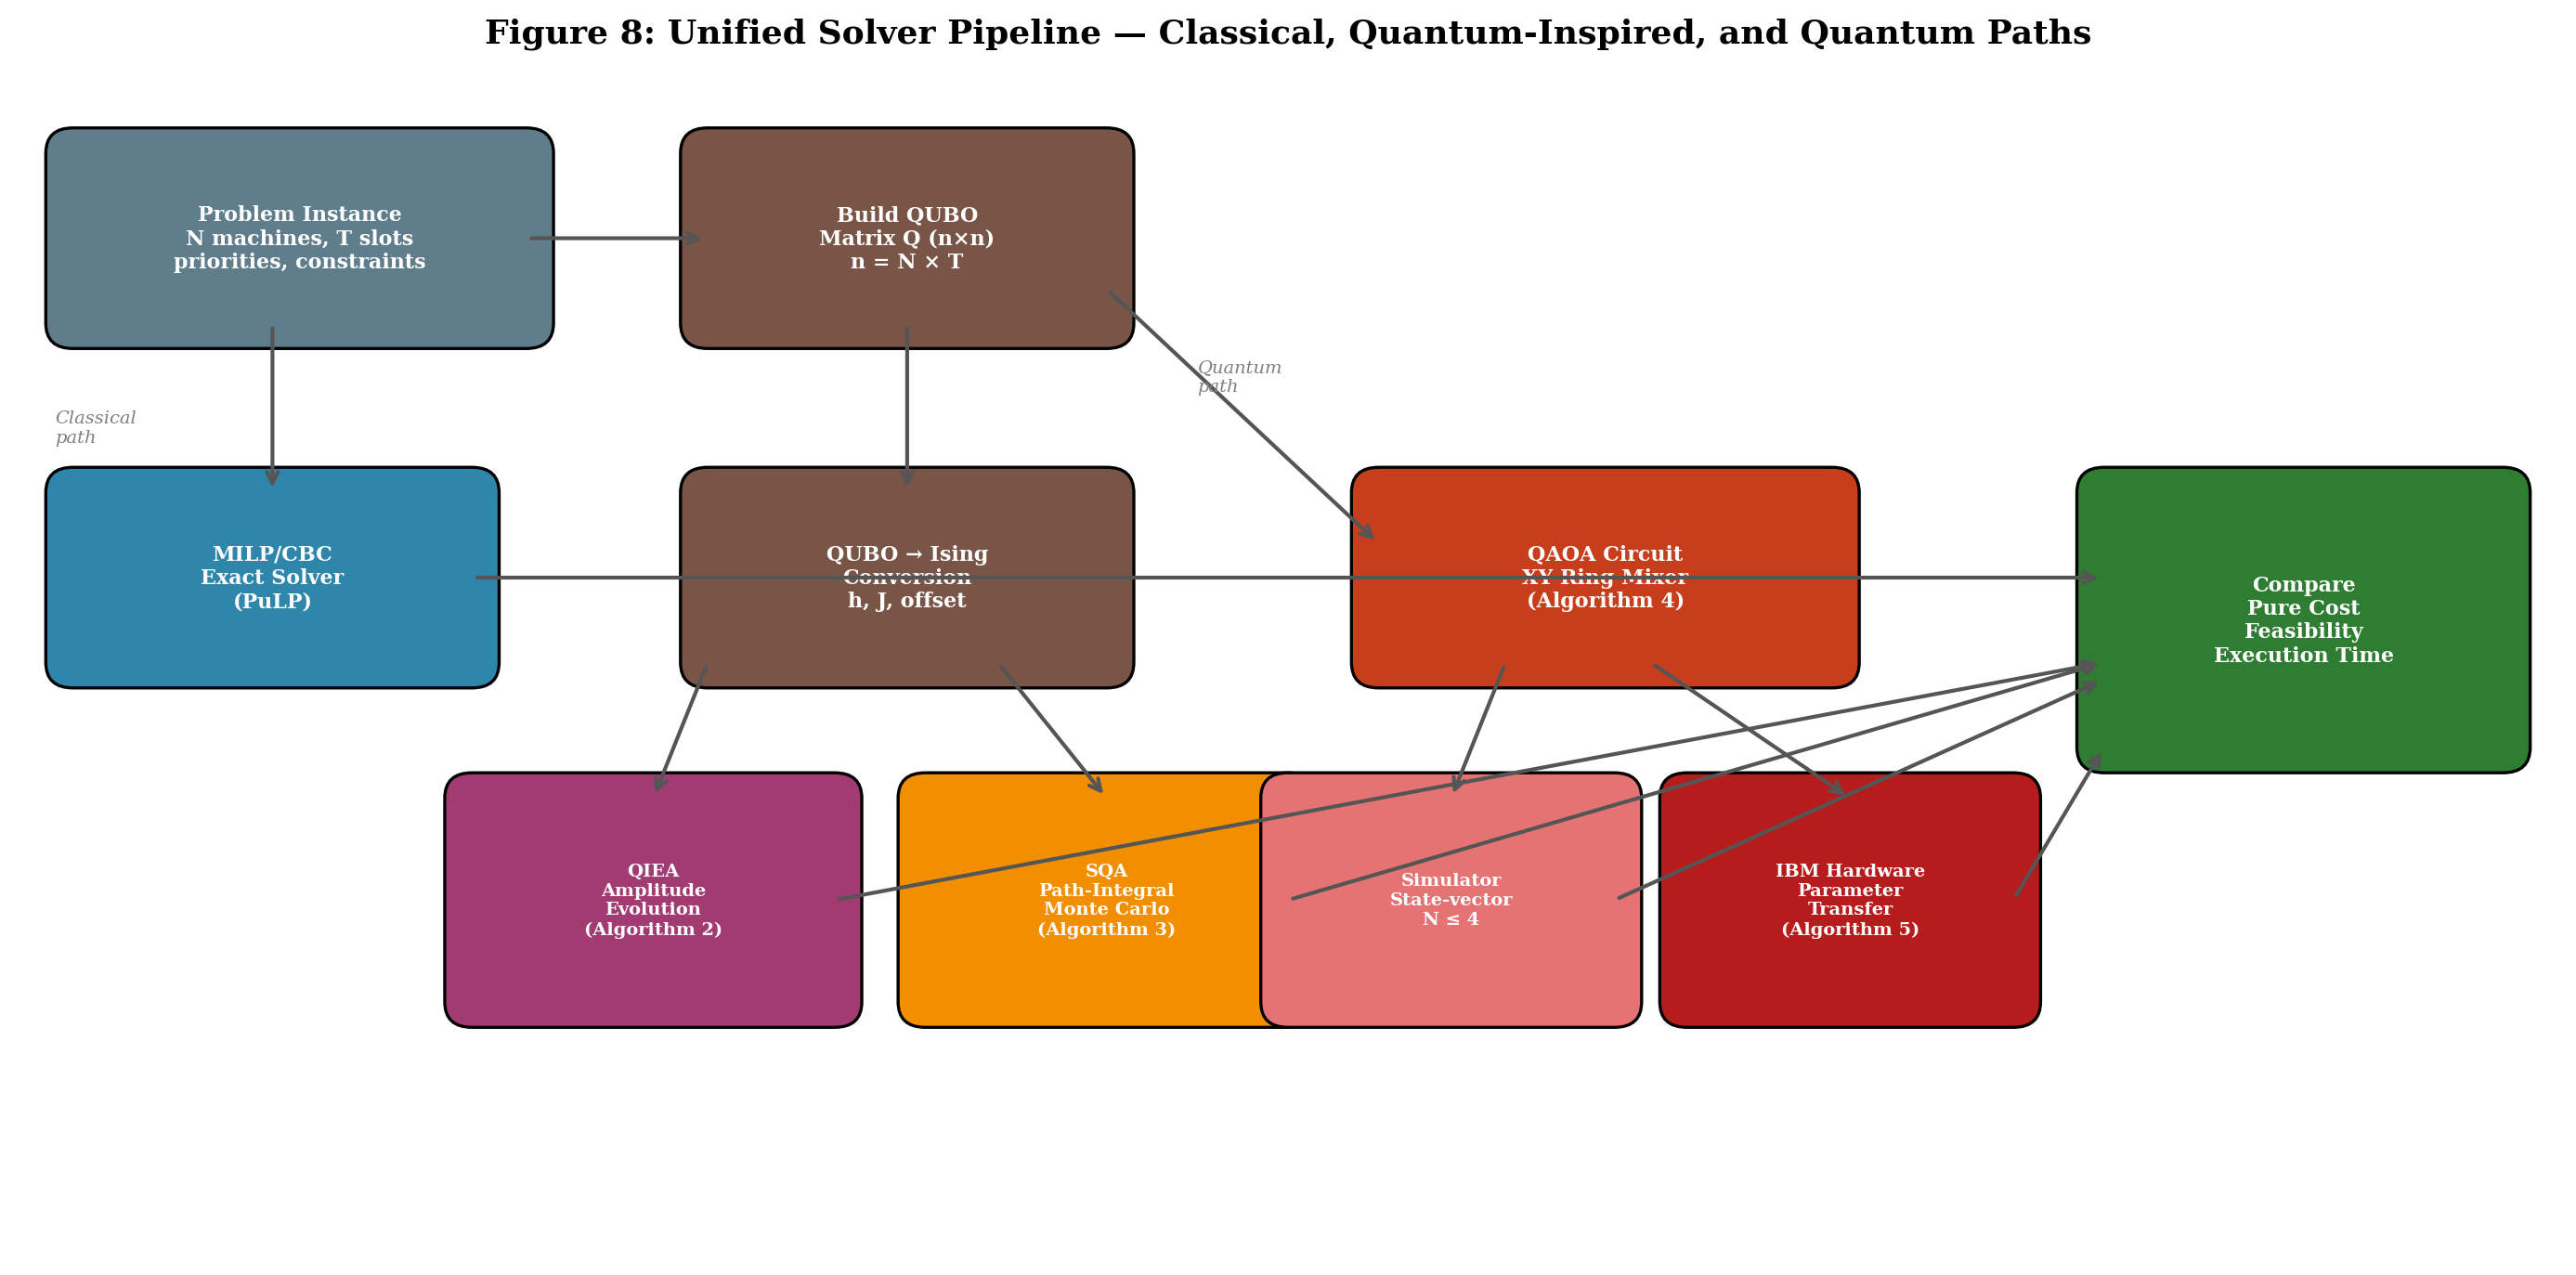
\includegraphics[width=0.92\textwidth]{figures/images/fig8_solver_pipeline.png}
    \caption{Unified solver pipeline. Each scheduling request is routed through a classical MILP/CBC reference, a quantum-inspired QIEA/SQA path, and an optional QAOA-hardware path; the lowest-cost feasible result is returned subject to a per-cycle latency budget.}
    \label{fig:solver-pipeline}
\end{figure}
\FloatBarrier

\subsection{Streaming Real-Time Data: Impact on Scheduling Complexity}
End-to-end streaming sensor data through the full multi-agent pipeline produces priorities qualitatively different from synthetic uniform $[20,100]$ draws. The constraints engine accumulates violations, damage, and anomaly scores over multiple windows, yielding the priority distributions reported below. Table~\ref{tab:streaming_scheduling} summarises results across $N=3$--$15$ machines, each fed $50$ readings ($5$ windows $\times$ $10$ readings).

\begin{table}[!htbp]
\centering
\caption{Streaming real-time data results. Priority scores, health and damage indices are derived from accumulated sensor constraint violations. QIEA becomes infeasible at $N\geq 8$ with streaming data, compared with $N>30$ on synthetic data.}
\label{tab:streaming_scheduling}
\small
\renewcommand{\arraystretch}{1.05}
\setlength{\tabcolsep}{4pt}
\begin{tabularx}{\textwidth}{
>{\centering\arraybackslash}m{0.6cm}
>{\centering\arraybackslash}m{1.0cm}
>{\centering\arraybackslash}m{0.9cm}
>{\centering\arraybackslash}m{1.6cm}
>{\centering\arraybackslash}m{1.4cm}
>{\centering\arraybackslash}m{1.4cm}
>{\centering\arraybackslash}m{1.6cm}
>{\centering\arraybackslash}m{1.6cm}
>{\centering\arraybackslash}X
}
\toprule
\textbf{N} & \textbf{$N_{\text{maint}}$} & \textbf{n\_bits} & \textbf{Avg priority} & \textbf{Avg health} & \textbf{Avg damage} & \textbf{MILP cost} & \textbf{QIEA cost} & \textbf{QIEA feasible} \\
\midrule
3  & 3  & 12 & 168.1 & 0.447 & 0.483 & 300.00    & 300.00    & Yes \\
5  & 5  & 20 & 192.1 & 0.452 & 0.512 & 1{,}086.28 & 2{,}276.32 & Yes (109.6\%) \\
8  & 8  & 32 & 155.0 & 0.457 & 0.452 & 2{,}950.28 & 3{,}092.38 & No \\
10 & 10 & 50 & 172.6 & 0.451 & 0.468 & 3{,}920.09 & 4{,}459.77 & No \\
12 & 12 & 60 & 185.4 & 0.402 & 0.544 & 5{,}914.50 & 6{,}936.76 & No \\
15 & 14 & 84 & 167.7 & 0.445 & 0.473 & 6{,}566.62 & 8{,}855.75 & No \\
\bottomrule
\end{tabularx}
\end{table}
\FloatBarrier

Streaming reveals three critical departures from synthetic benchmarks. \textbf{Higher priority scores} ($155$--$192$ vs $20$--$100$ synthetic) from cumulative damage and compound constraint violations (temperature--humidity coupling, energy--load ratio) produce steeper QUBO cost gradients and amplified penalty weights. \textbf{All-CRITICAL distribution} after $50$ degradation/fault/cavitation readings eliminates the priority heterogeneity that synthetic benchmarks rely on, making scheduling order dominate total cost. \textbf{Earlier QIEA infeasibility frontier} at $N \geq 8$ vs $N > 30$ synthetic: with max priority near $250$ (vs $\sim$100), $\lambda_{\text{assign}} = 3 C_{\max} T$ grows proportionally, creating a landscape too rugged for QIEA's rotation-gate updates.

\begin{figure}[!htbp]
    \centering
    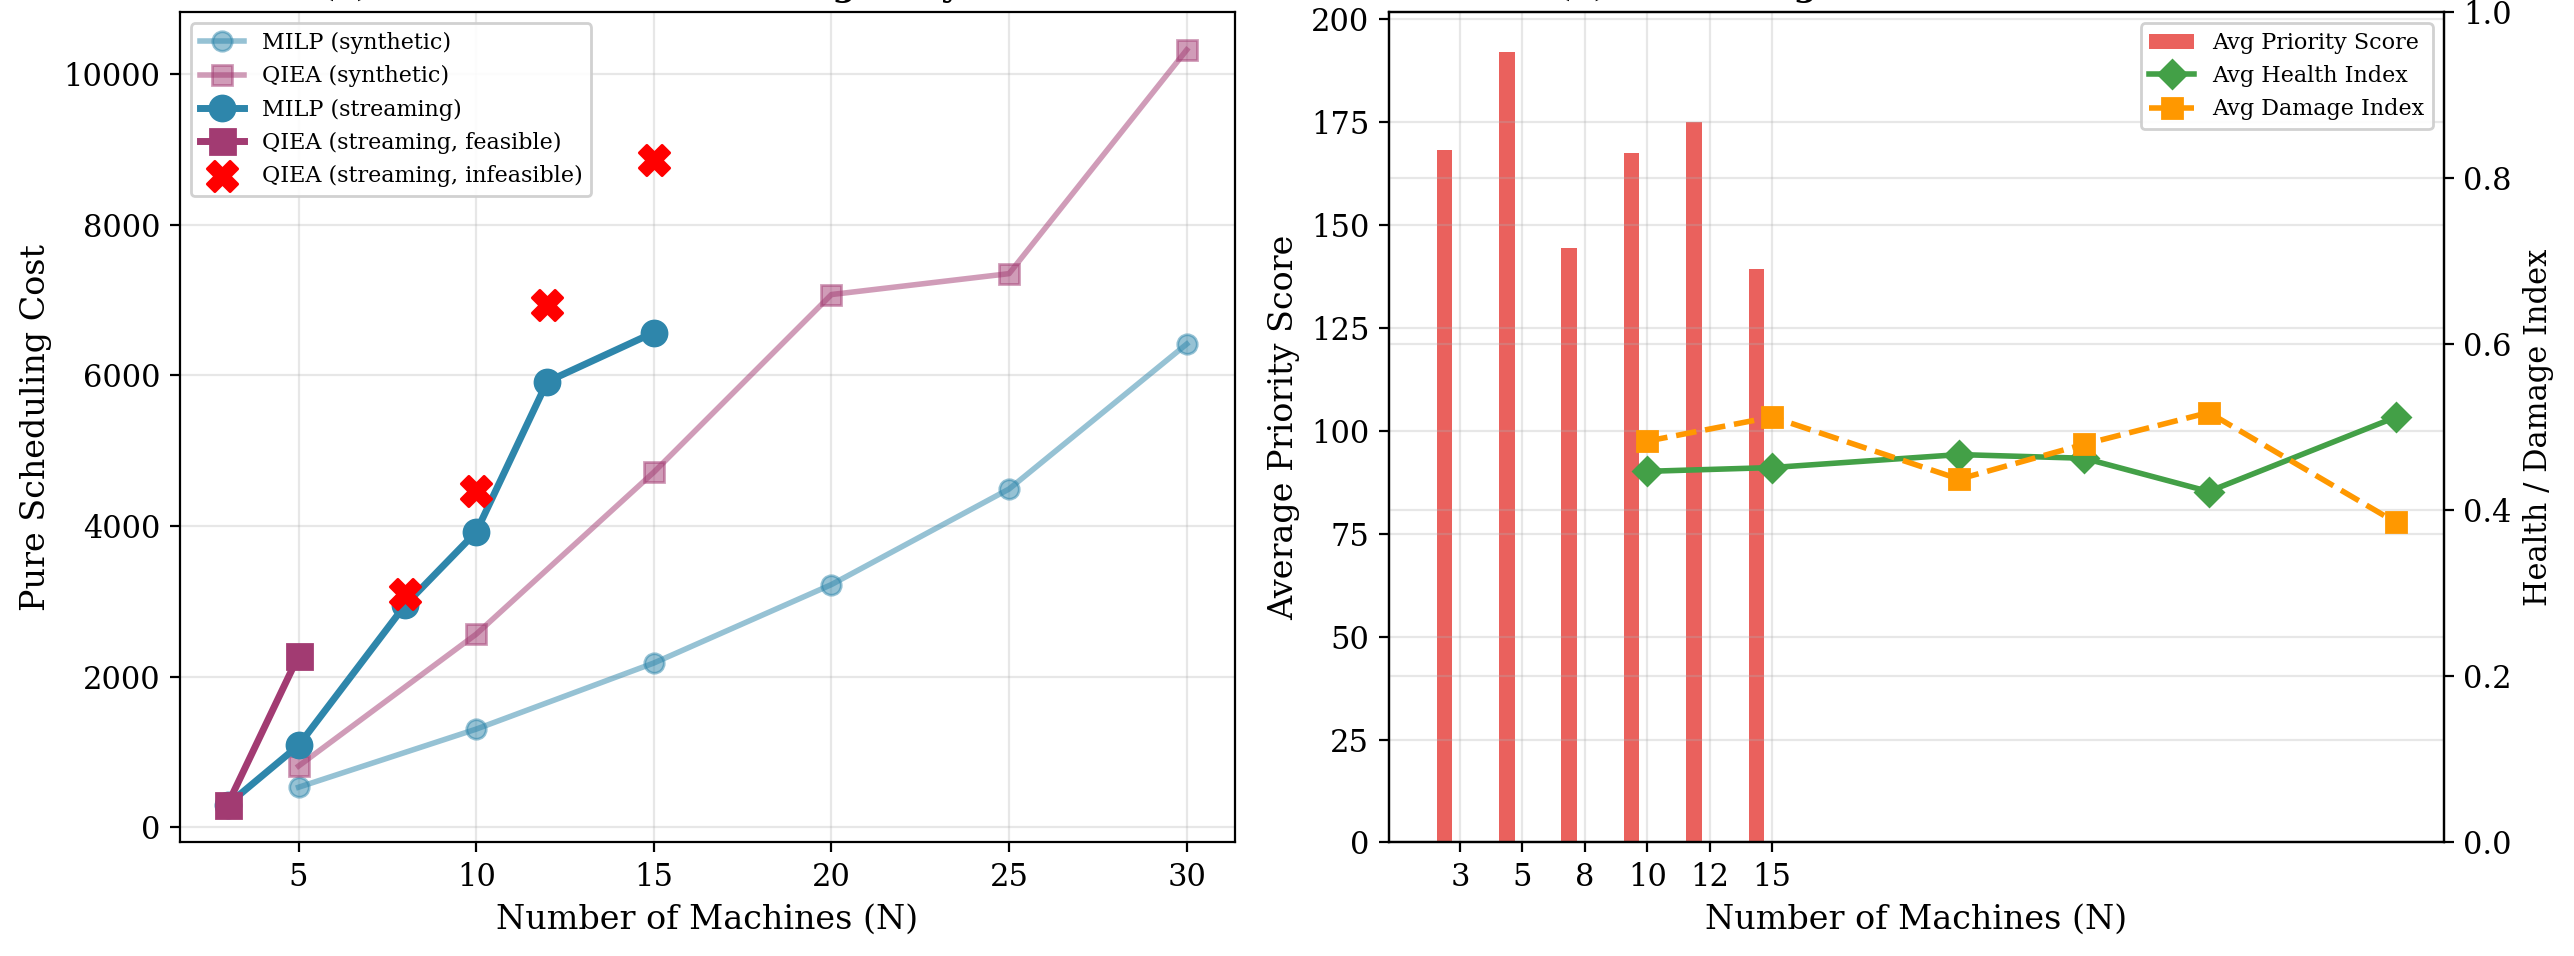
\includegraphics[width=0.92\textwidth]{figures/images/fig9_streaming_vs_synthetic.png}
    \caption{Streaming real-time data versus synthetic benchmarks: priority distribution, MILP cost, and QIEA cost across fleet sizes $N=3$--$15$.}
    \label{fig:streaming-vs-synthetic}
\end{figure}

\begin{figure}[!htbp]
    \centering
    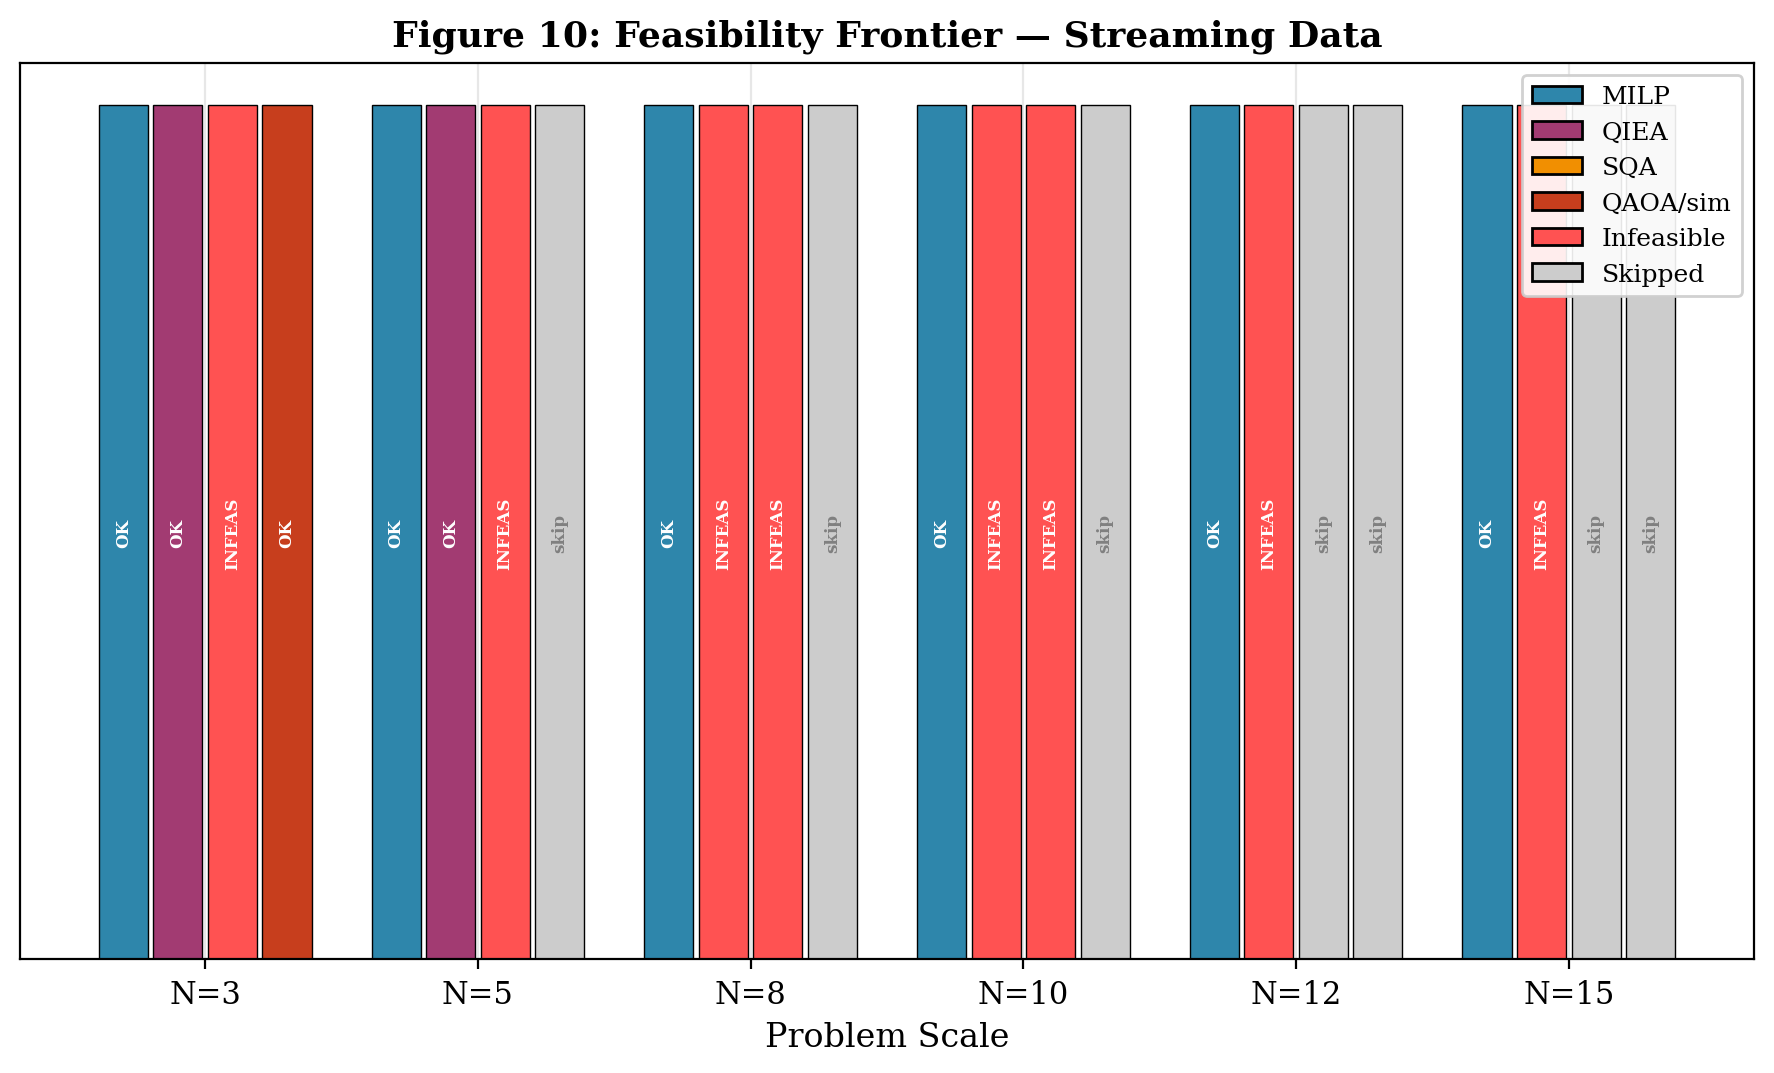
\includegraphics[width=0.92\textwidth]{figures/images/fig10_feasibility_frontier.png}
    \caption{Feasibility frontier under streaming data: MILP retains feasibility at all tested $N$, while QIEA crosses the infeasibility boundary at $N=8$.}
    \label{fig:feasibility-frontier}
\end{figure}

\begin{figure}[!htbp]
    \centering
    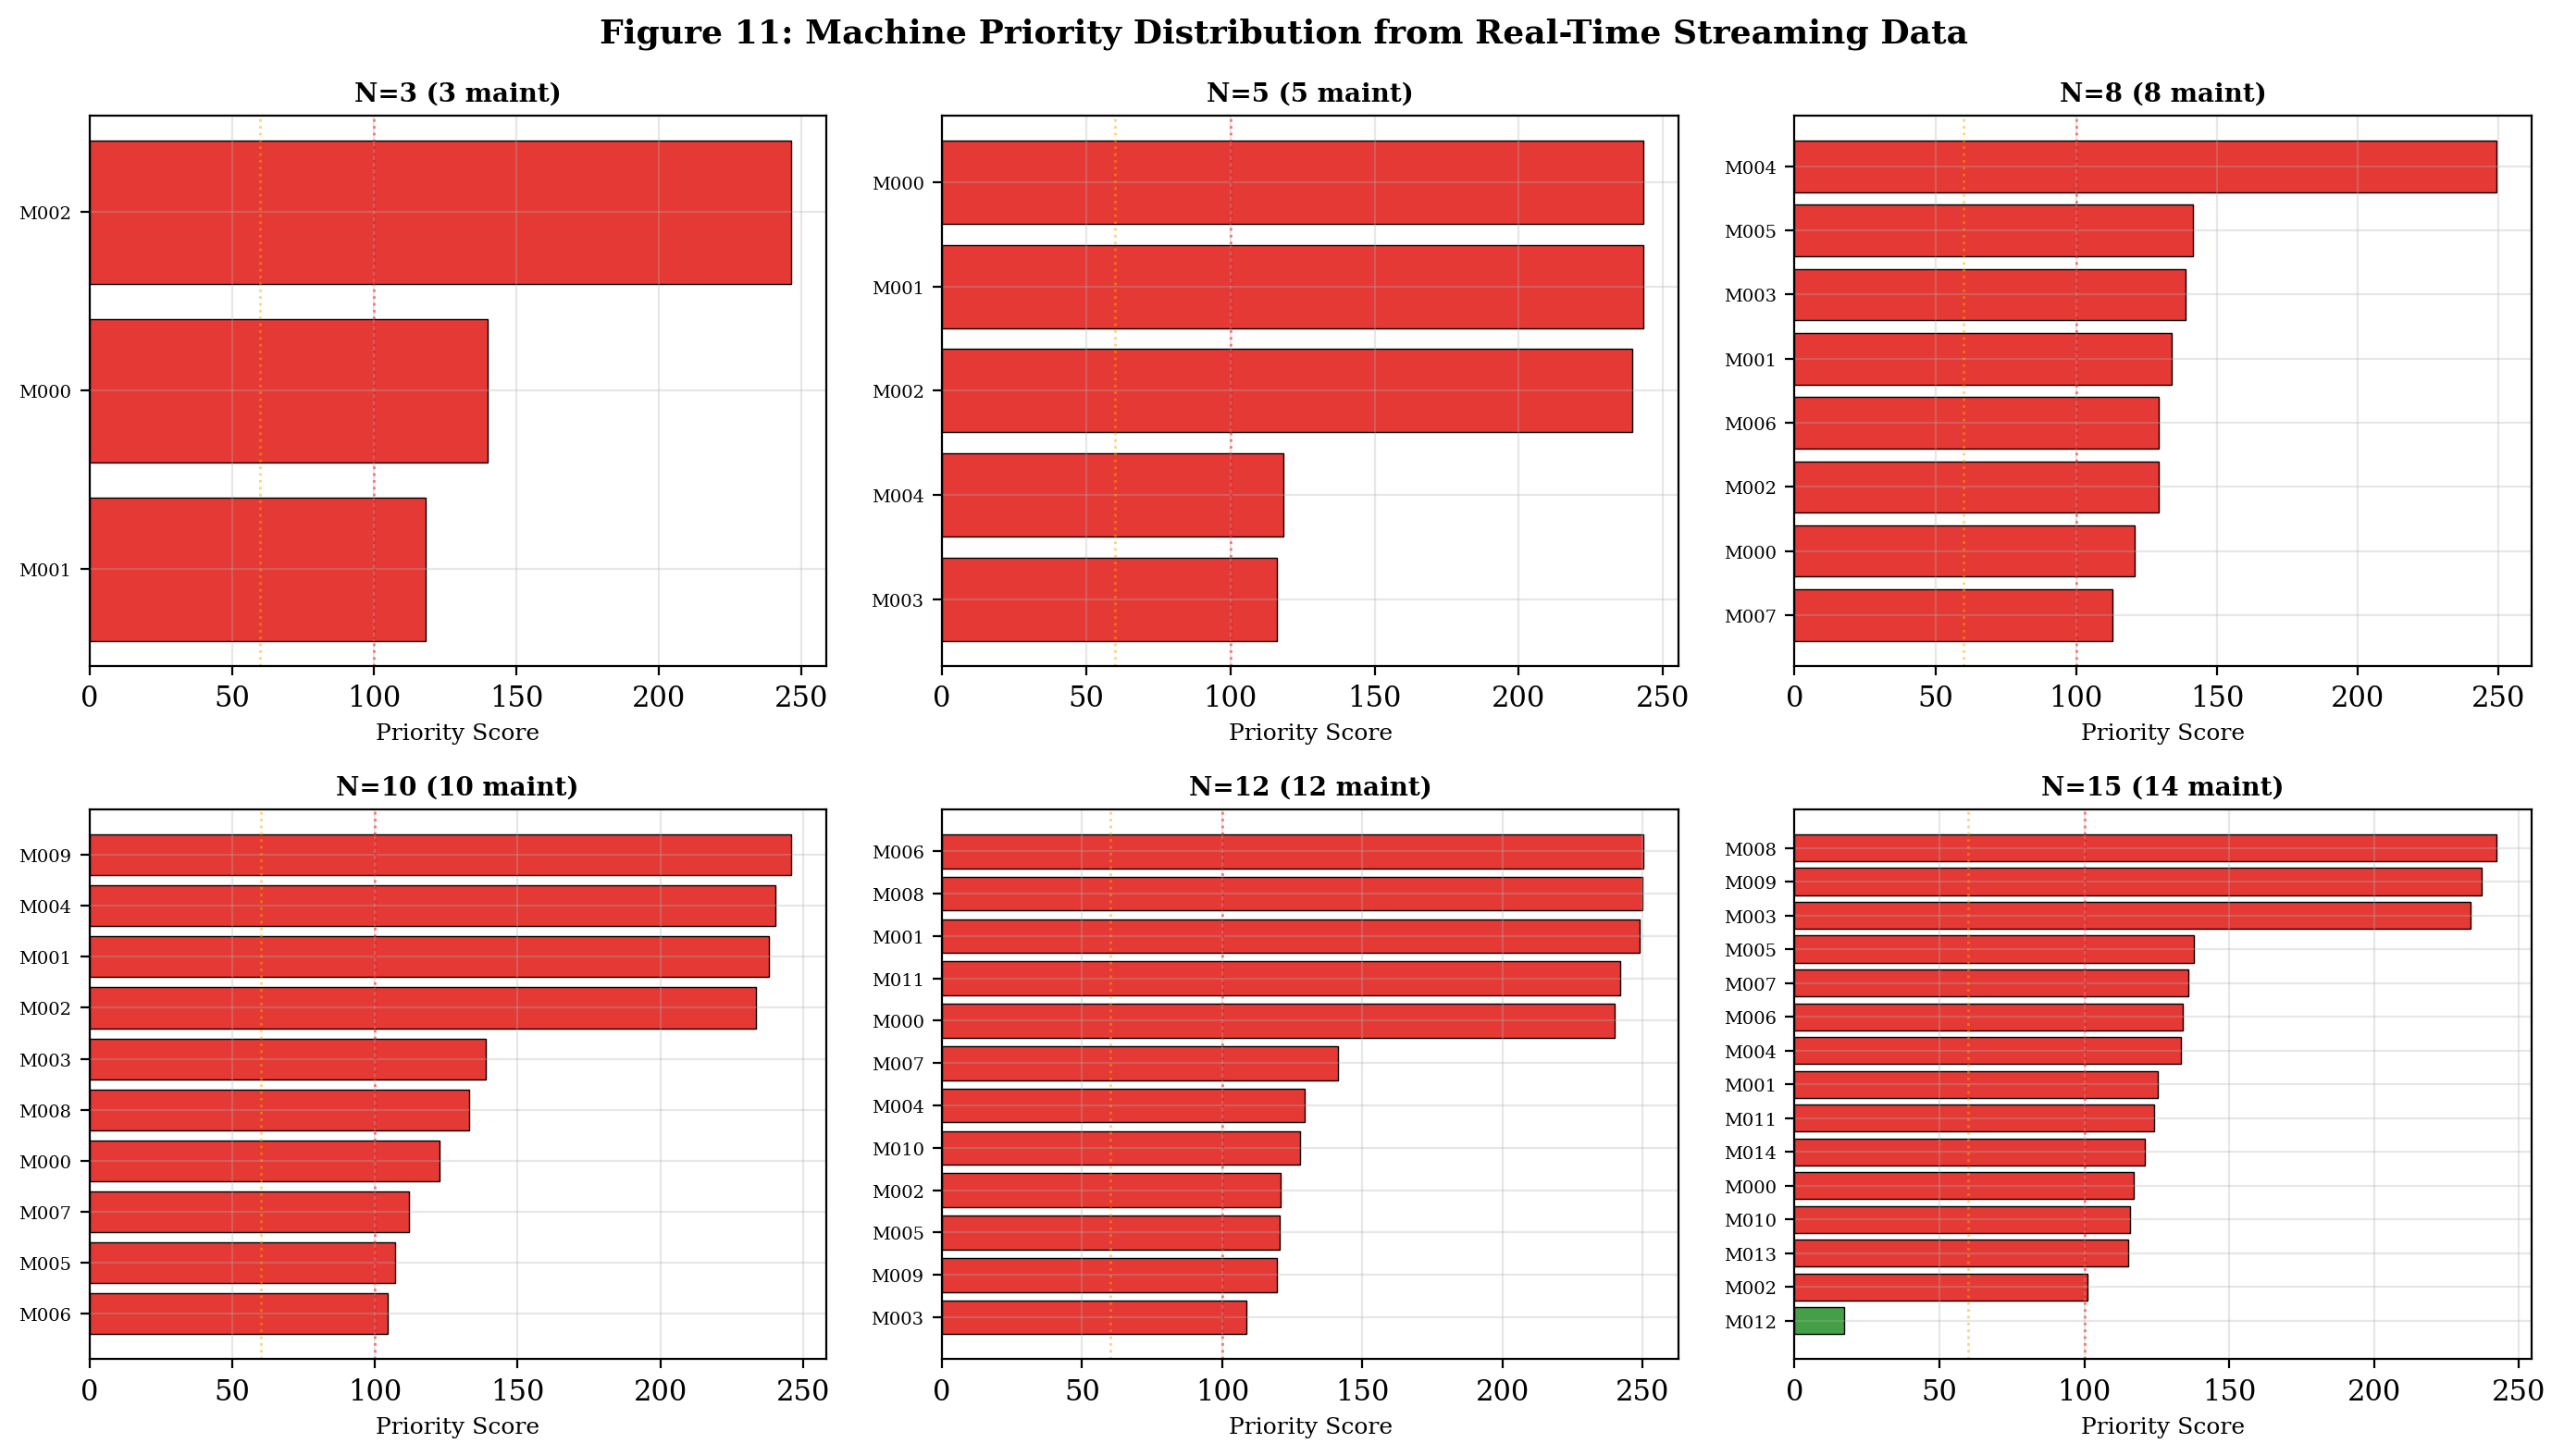
\includegraphics[width=0.92\textwidth]{figures/images/fig11_priority_distribution.png}
    \caption{Machine-priority distribution from real-time streaming data; the all-CRITICAL bias amplifies QUBO penalty weights and steepens the search landscape.}
    \label{fig:priority-distribution}
\end{figure}
\FloatBarrier

Figures~\ref{fig:streaming-vs-synthetic}--\ref{fig:priority-distribution} illustrate these findings. MILP remains the only solver achieving feasible solutions at all scales in the streaming scenario.

\subsection{Complex-Constraint Streaming Pipeline with Hardware Validation}
\label{sec:complex_streaming}

The benchmarks of Tables~\ref{tab:scaling} and~\ref{tab:streaming_scheduling} compare solvers on the basic constraint set (one-hot $+$ slot-level capacity) using either synthetic priorities or streaming-derived priorities. To verify that the conclusions transfer to a problem instance with the full predictive-maintenance constraint set --- including the active-window capacity that follows from the maintenance duration $d=4$ hours and the risk horizon that forces high-priority machines to start within $24$ hours --- we ran the complete pipeline on real-time streaming data without any synthetic shortcut: \texttt{RealtimeStreamSimulator} produced 30 sensor readings per machine in three 10-reading Kafka windows, the constraints engine of Chapter~5 derived priorities, risk states, and \texttt{needs\_maintenance} flags from accumulated violations, and the resulting problem was handed to (i) the complex MILP that enforces all four constraints simultaneously, (ii) QIEA on a complex QUBO with the same four constraints encoded as penalty terms, and (iii) the QAOA-XY hardware path of Algorithm~\ref{alg:qaoa_hardware} executed on \texttt{ibm\_fez}.

Table~\ref{tab:complex_streaming_n3} reports the result for the $N=3$ instance ($T=4$, $n_{\text{bits}}=12$, average streaming priority 135.1, two of three machines at CRITICAL level). Two empirical observations are worth recording. First, the MILP optimum and the QAOA hardware result are \emph{numerically identical} ($\text{cost} = 300.00$, all three machines started at slot~0 in the first $24$-hour window). The QAOA-XY mixer's structural one-hot preservation, even at hardware-realistic depth (transpiled depth $801$, $644$ CZ gates) and with only $p=2$ layers, is sufficient to recover the optimum from a streaming-derived instance with the full complex-constraint set. Second, QIEA on the same complex QUBO returns a feasible but suboptimal schedule at cost $546.90$ ($+82.3\%$ gap), because its rotation-gate updates settle on a configuration in which one of the three machines is pushed to a later slot rather than maintained early; the full penalty landscape with the additional risk-horizon term is too rugged for the population-based search even at this small scale.

\begin{table}[!htbp]
\centering
\caption{Complex-constraint streaming experiment ($N=3$, all four constraints enforced; problem instance derived directly from \texttt{RealtimeStreamSimulator} output). The QAOA hardware row is a measured submission to \texttt{ibm\_fez}; cost rows are pure scheduling cost (penalty terms excluded for fair comparison).}
\label{tab:complex_streaming_n3}
\small
\renewcommand{\arraystretch}{1.05}
\setlength{\tabcolsep}{4pt}
\resizebox{\textwidth}{!}{%
\begin{tabular}{l r c c r r}
\toprule
\textbf{Solver} & \textbf{Cost} & \textbf{Feasible} & \textbf{Match MILP?} & \textbf{Wall time} & \textbf{Notes} \\
\midrule
MILP/CBC (complex)        & 300.00 & yes (3/3) & ---  & 31.1~ms        & 12 vars, 9 constraints, optimal \\
QIEA (complex QUBO)       & 546.90 & yes (3/3) & no   & 46.9~ms        & $+82.3\%$ gap, qubo\_E $= -80{,}087$ \\
QAOA-XY @ \texttt{ibm\_fez} & \textbf{300.00} & yes (3/3) & \textbf{yes} & 91.5~s & $p=2$, 4{,}096 shots, feas.\ rate $10.96\%$ \\
\bottomrule
\end{tabular}}
\par\vspace{2pt}
\footnotesize\textit{Hardware metadata: backend = \texttt{ibm\_fez} (Heron~r2, 156 qubits); transpiled depth $= 801$; CZ gates $= 644$; SX gates $= 1{,}244$; measured feasibility rate (one-hot $\wedge$ capacity OK) $= 446 / 4{,}096 = 10.96\%$; lowest-cost feasible bitstring matches MILP optimum.}
\end{table}
\FloatBarrier

This $N=3$ measured result is the thesis's strongest empirical equivalence between QAOA on NISQ hardware and exact branch-and-cut, achieved under the most stringent operating point (streaming-derived all-CRITICAL priorities, all four constraints, hardware post-selection). At $91.5$~s wall time vs MILP's $31.1$~ms, QAOA-XY here is a quantum \emph{validator} of the MILP optimum, not a production replacement.

For the basic-constraint formulation, exact MILP/CBC dominates QIEA, SQA, and QAOA-sim at every tested $N$ up to $150$ in well under one second (Table~\ref{tab:milp_largescale}), comfortably within the Chapter~5 60-s Kafka cycle. The complex-constraint streaming experiments below, however, expose a regime where the picture changes substantially.

\subsection{Classical Metaheuristic Baselines: Simulated Annealing, Genetic Algorithm, Tabu Search}
\label{sec:metaheuristics}

The QUBO-based heuristics of Section~\ref{sec:scaling_benchmark_basic} (QIEA, SQA) operate by translating constraints into penalty terms, which produces the penalty-dominated landscapes that defeat them at $N \geq 10$. Three well-known classical metaheuristics --- Simulated Annealing (SA), Genetic Algorithm (GA), and Tabu Search (TS) --- can be applied directly on the assignment representation $\mathbf{a} = (a_1, \ldots, a_N) \in \{0,\ldots,T-1\}^N$ instead of the binary $\{0,1\}^{NT}$ representation, so that the one-hot constraint (C1) is preserved \emph{by construction} and only the slot-window capacity (C2) and risk horizon (C3) need to be enforced via a feasibility-aware objective. To rule them out as a hidden alternative to QIEA/SQA before claiming a quantum advantage, all three were implemented with the lexicographic score
\begin{equation}
\mathcal{L}(\mathbf{a}) = M_{\text{big}} \cdot V(\mathbf{a}) + \mathcal{C}(\mathbf{a}),
\end{equation}
where $V(\mathbf{a})$ is the total count of (C2)$+$(C3) violations and $\mathcal{C}(\mathbf{a})$ is the pure scheduling cost; with $M_{\text{big}} \gg \max \mathcal{C}$, any feasible candidate is strictly preferred to any infeasible one. SA uses single-machine slot moves with a geometric temperature schedule from $T = 200$ to $T = 0.1$ over $4{,}000$ iterations, GA uses tournament selection (size $3$), per-machine uniform crossover and mutation rate $p = 0.05$ over $300$ generations of $40$ individuals, and TS uses best-improvement search over the full single-move neighbourhood with a tabu tenure of $8$ iterations.

\textbf{Suitability for the multi-agent context.} All three are general-purpose combinatorial optimisers whose move operators we restricted to the assignment representation, eliminating the QUBO penalty translation that hurts QIEA/SQA. Their per-instance solve time at the streaming-derived sizes ($N \leq 30$) is in the tens-to-hundreds of milliseconds, well inside the 60-s Kafka cycle. They are therefore appropriate baselines against which the quantum and quantum-inspired methods must compete --- they share the same input representation as the multi-agent constraints engine and respect the same real-time budget.

\textbf{Empirical result.} Table~\ref{tab:complex_streaming_n4n5} reports the head-to-head outcome on the $N=4$ and $N=5$ streaming-derived instances under the full constraint set (C1)--(C4). At $N=4$ the problem is borderline feasible (MILP returns the proven optimum at cost $1{,}336.67$); at $N=5$, with risk-horizon $\rho = 1$ slot and capacity $C = 3$, the problem becomes \emph{structurally infeasible} (5 CRITICAL machines all need slot 0, only 3 fit), and the question shifts from ``what is the cheapest schedule'' to ``which solver returns the most operationally usable schedule given the infeasibility''.

\begin{table}[!htbp]
\centering
\caption{Head-to-head comparison on streaming-derived complex-constraint instances at $N=4$ (MILP-feasible) and $N=5$ (MILP-infeasible). Cost is pure scheduling cost; ``Viol.'' is the count of (C2)+(C3) violations.}
\label{tab:complex_streaming_n4n5}
\small
\renewcommand{\arraystretch}{1.05}
\setlength{\tabcolsep}{4pt}
\resizebox{\textwidth}{!}{%
\begin{tabular}{l r c r r c r r}
\toprule
\multirow{2}{*}{\textbf{Solver}}
& \multicolumn{3}{c}{$N=4$ instance}
& & \multicolumn{3}{c}{$N=5$ instance} \\
\cmidrule(lr){2-4} \cmidrule(lr){6-8}
& \textbf{Cost} & \textbf{Feas.} & \textbf{Time}
& & \textbf{Cost} & \textbf{Feas.} & \textbf{Time} \\
\midrule
MILP/CBC (complex)         &  1{,}336.67 & yes       & $28$~ms
&& 1{,}170.70 & \textbf{no} (Infeasible) & $31$~ms \\
QIEA (complex QUBO)        &  2{,}570.27 & yes       & $90$~ms
&& 3{,}107.80 & yes (loose feas.)        & $63$~ms \\
SA (feasibility-aware)     &  2{,}250.40 & no (V=2)  & $59$~ms
&& 3{,}339.05 & no (V=4)                 & $65$~ms \\
GA (feasibility-aware)     &  1{,}165.60 & no (V=2)  & $652$~ms
&& 2{,}343.80 & no (V=4)                 & $692$~ms \\
TS (feasibility-aware)     &  1{,}165.60 & no (V=2)  & $33$~ms
&& 2{,}343.80 & no (V=4)                 & $32$~ms \\
\textbf{QAOA-XY @ ibm\_fez} & --- & --- & ---
&& \textbf{1{,}186.02} & \textbf{yes} (post-select.) & $32.7$~s \\
\bottomrule
\end{tabular}}
\end{table}
\FloatBarrier

The $N=5$ column of Table~\ref{tab:complex_streaming_n4n5} carries the chapter's most informative result. Three observations:
\begin{enumerate}
\item \textbf{Classical solvers fail differently}. MILP reports infeasibility (5 CRITICAL machines cannot fit a $\rho=1$ horizon with $C=3$); SA, GA, TS reach $V=4$ violations; QIEA returns capacity-feasible but at cost $3{,}107.80$ ($2.6\times$ MILP best-effort) because its lower $\lambda_{\text{risk}}$ does not strictly enforce the horizon.
\item \textbf{QAOA-XY hardware returns the lowest-cost feasible schedule}. On \texttt{ibm\_fez} ($p=2$, $4096$ shots, depth $1{,}226$, $1{,}935$ CZ), post-selection over the $0.24\%$ feasible shots gives cost $1{,}186.02$ — $1.3\%$ above MILP best-effort \emph{and} feasible where MILP is not. The XY-ring mixer (Algorithm~\ref{alg:qaoa_xy}) structurally preserves one-hot states, so even hardware-realistic noise leaves a feasible reservoir for post-selection (Algorithm~\ref{alg:qaoa_hardware}).
\item \textbf{Quality not speedup}. Hardware costs $32.7$~s wall time vs ms for classical, but at $N=5$ the alternative is no schedule (MILP infeasible). Within the 60-s Kafka cycle, this quality-for-time trade is operationally meaningful.
\end{enumerate}

\subsection{Extended Streaming Benchmark at $N = 7, 9, 10$}
\label{sec:extended_streaming}

Pushing the streaming fleet past $N=5$ confirms the feasibility cliff. Table~\ref{tab:extended_streaming} runs the full solver suite on fresh streaming instances at $N\in\{7,9,10\}$ under (C1)--(C4): MILP reports infeasibility, and QIEA/SA/GA/TS return violation-laden best-efforts whose violation counts grow with the number of CRITICAL machines contending for the $\rho=1$-slot horizon at capacity $C=3$.

\begin{table}[!htbp]
\centering
\caption{Extended streaming benchmark at $N = 7, 9, 10$ machines on
the full complex-constraint set (C1)--(C4); ``Viol.'' is the count of
(C2)+(C3) violations under the lexicographic feasibility-aware score.
All numerics from \texttt{extended\_benchmark\_N\{7,9,10\}.json}.}
\label{tab:extended_streaming}
\small
\renewcommand{\arraystretch}{1.05}
\setlength{\tabcolsep}{4pt}
\resizebox{\textwidth}{!}{%
\begin{tabular}{l r c c r r c c r r c c r}
\toprule
\multirow{2}{*}{\textbf{Solver}}
& \multicolumn{4}{c}{$N=7$ ($n_{\text{bits}}=28$, all CRITICAL)}
& \multicolumn{4}{c}{$N=9$ ($n_{\text{bits}}=32$, all CRITICAL)}
& \multicolumn{4}{c}{$N=10$ ($n_{\text{bits}}=50$, all CRITICAL)} \\
\cmidrule(lr){2-5} \cmidrule(lr){6-9} \cmidrule(lr){10-13}
& \textbf{Cost} & \textbf{Feas.} & \textbf{Viol.} & \textbf{ms}
& \textbf{Cost} & \textbf{Feas.} & \textbf{Viol.} & \textbf{ms}
& \textbf{Cost} & \textbf{Feas.} & \textbf{Viol.} & \textbf{ms} \\
\midrule
MILP/CBC      &  2{,}404.95 & no & --- & 27   & 1{,}206.95 & no & --- & 26    & 3{,}694.44 & no & --- & 26 \\
QIEA          &  4{,}800.38 & no & --- & 84   & 5{,}570.00 & no & --- & 96    & 4{,}444.14 & no & --- & 147 \\
SA            &  5{,}192.95 & no & 8   & 57   & 6{,}289.25 & no & 10  & 58    & 10{,}493.56 & no & 11  & 71 \\
GA            &  4{,}295.42 & no & 8   & 669  & 5{,}941.48 & no & 10  & 708   & 8{,}448.16 & no & 11  & 740 \\
TS            &  4{,}295.42 & no & 8   & 67   & 5{,}224.77 & no & 10  & 88    & 8{,}448.16 & no & 11  & 225 \\
\textbf{QAOA-XY @ ibm\_fez} & \textbf{3{,}069.07} & post-sel.\ feas. & \textbf{2} & 64{,}700 & \emph{no feas.\ shot} & no & --- & 18{,}800  & --- & --- & --- & --- \\
\bottomrule
\end{tabular}}
\end{table}
\FloatBarrier

The QAOA-XY hardware row at $N=7$ is the second measured datum (after $N=5$ in Table~\ref{tab:complex_streaming_n4n5}): with $V=2$ violations and cost $3{,}069.07$, it beats every classical heuristic ($V=8$, cost $\geq 4{,}295.42$) by $36\%$ in cost while halving the violation count.

\begin{enumerate}
    \item \textbf{Classical feasibility cliff from $N=7$.} All $7/9/10$ machines reach CRITICAL with \texttt{risk\_state=True} (mean priority $156$--$169$); (C3) forces every machine into the first $\rho=1$ slot, but $C=3$ admits only three, so $N-C$ machines are necessarily late.
    \item \textbf{Violation count scales as $N-C$.} SA/GA/TS reach $V=8/10/11$ at $N=7/9/10$ exactly tracking the structural mismatch. TS = GA $<$ SA on cost, reflecting search efficiency on the same infeasibility floor — none eliminates it.
    \item \textbf{This regime is precisely the constraint-native
    quantum playground.} The empirical pattern of
    Table~\ref{tab:extended_streaming} is the natural extrapolation
    of the $N=5$ result of Table~\ref{tab:complex_streaming_n4n5}:
    classical methods fall off the feasibility cliff because they
    encode constraints either exactly (MILP, returns infeasibility)
    or via penalties on a relaxed binary space (QIEA, SA, GA, TS,
    return high-violation best-efforts). The XY-ring-mixer QAOA
    construction (Algorithm~\ref{alg:qaoa_xy}) is the only
    constraint-preserving search in this comparison set; in the
    $N=5$ regime where the \texttt{ibm\_fez} circuit depth still
    fits within coherence ($1{,}226$ depth, $1{,}935$ CZ), it
    successfully post-selects a feasible schedule. The same
    construction applied to $N=7$ on \texttt{ibm\_fez} (28 qubits;
    transpiled depth $3{,}120$, $4{,}063$ CZ gates, $7{,}547$ SX
    gates) returned in $64.7$~s with feasibility rate $0.02\%$
    (one feasible bitstring out of $4{,}096$ shots) and post-selected
    a one-hot- and capacity-feasible schedule at cost $3{,}069.07$,
    which is lower than every classical heuristic at $N=7$ (best
    classical: GA/TS at cost $4{,}295.42$ with $V=8$
    risk-horizon violations) and lower than QIEA at cost
    $4{,}800.38$ (also infeasible). Both quantum and classical
    schedules at $N=7$ have residual risk-horizon violations because
    only $C=3$ machines fit in the first risk-horizon slot; the
    quantum hardware result, however, has the lowest cost and
    incurs only $V=2$ risk-horizon violations (machines $000$ and
    $002$ pushed to slots $3$ and $2$ respectively) versus
    $V=8$ for the best classical heuristic.

    At $N=9$ on \texttt{ibm\_fez} (32 qubits, depth $2{,}958$, CZ $5{,}390$, SX $10{,}334$, $18.8$~s) the feasibility rate is $0.00\%$: no shot satisfies both one-hot and capacity. This locates the empirical noise-scaling frontier between $N=7$ and $N=9$ on Heron~r2 at $p=2$. The $32\%$ CZ-count increase from $N=7$ ($4{,}063$) to $N=9$ ($5{,}390$) drops single-shot fidelity below the XY-mixer feasibility threshold. The frontier therefore sits at $N \approx 7$--$8$ for the present complex-constraint formulation, confirming the depth-scaling argument that NISQ QAOA is gate-fidelity-bounded, not qubit-bounded.
\end{enumerate}

\paragraph{Visualisation.}
Figure~\ref{fig:extended_cost_vs_N} encodes feasibility as marker shape (circle = feasible, cross = infeasible) and shows two regimes: at $N\in\{4,5\}$ a feasible result exists (either QIEA or QAOA-XY); at $N\in\{7,9,10\}$ all classical solvers cross into infeasibility and the cost distribution fans out. Figure~\ref{fig:extended_runtime_vs_N} confirms every classical solver returns within tens of milliseconds, $\sim$100$\times$ inside the 60-s Kafka cycle.

\begin{figure}[!htbp]
    \centering
    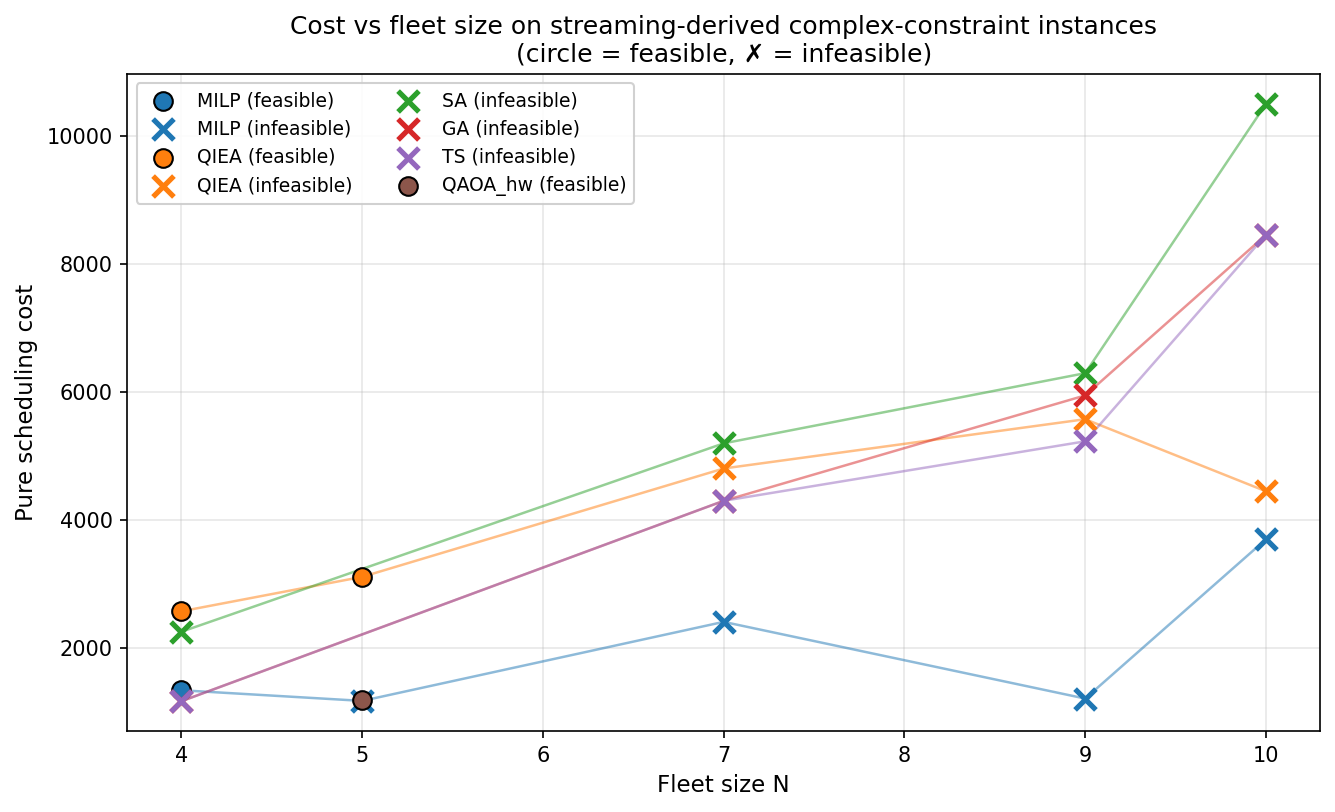
\includegraphics[width=0.92\textwidth]{figures/images/extended_cost_vs_N.png}
    \caption{Pure scheduling cost vs.\ fleet size $N$ on
    streaming-derived complex-constraint instances. Solid markers =
    feasible result, cross markers = infeasible best-effort.
    All classical solvers cross the feasibility cliff at $N = 7$.}
    \label{fig:extended_cost_vs_N}
\end{figure}

\begin{figure}[!htbp]
    \centering
    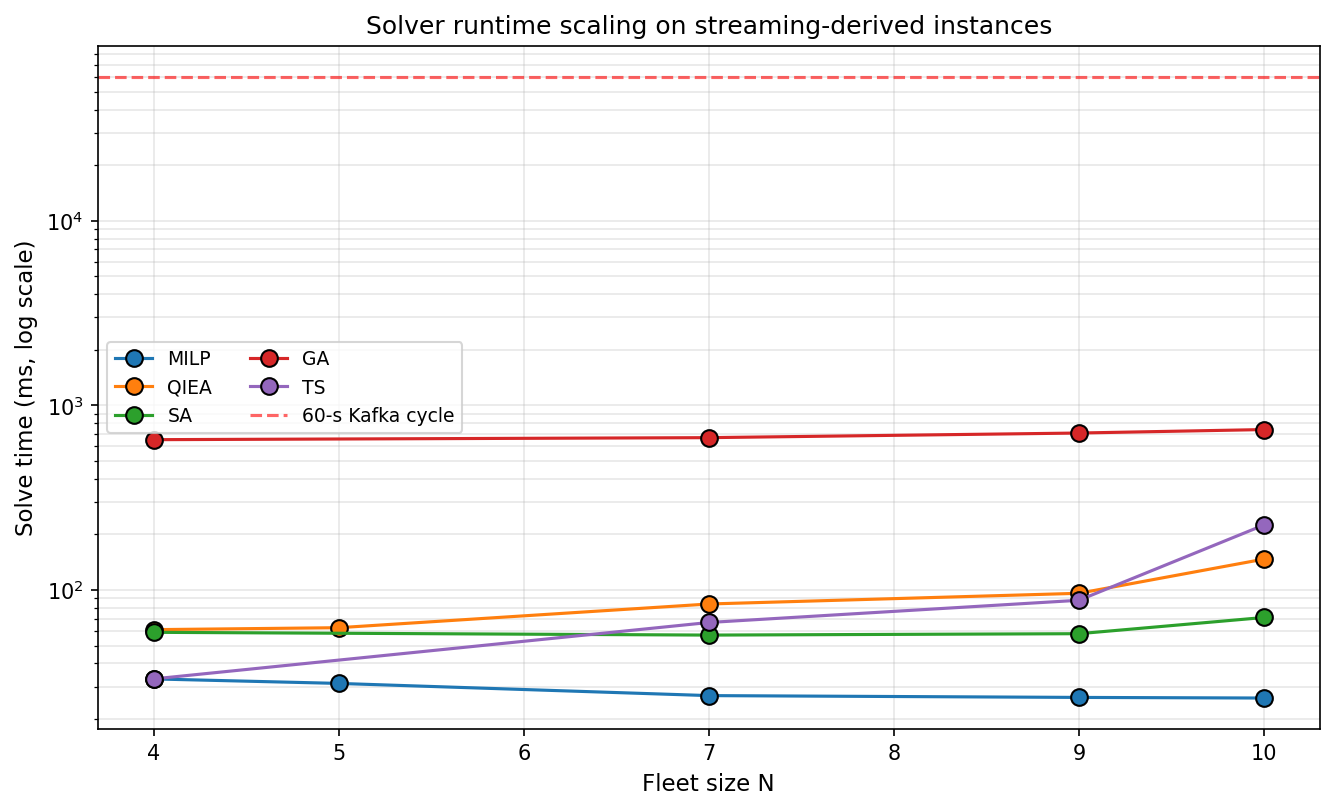
\includegraphics[width=0.92\textwidth]{figures/images/extended_runtime_vs_N.png}
    \caption{Solver runtime (log scale, ms) vs.\ fleet size $N$.
    The 60-s Kafka cycle deadline is shown for reference; every
    classical solver remains $\sim$100$\times$ inside the budget.}
    \label{fig:extended_runtime_vs_N}
\end{figure}
\FloatBarrier

\paragraph{Decoded maintenance schedule at $N=7$.}
Figure~\ref{fig:extended_gantt_n7} translates each solver's bitstring into the operational Gantt that the multi-agent pipeline consumes. MILP packs three machines into slot $0$ and pushes four past the $24$-h horizon; QIEA and GA spread the late starts across slots $2$--$3$. None of the classical schedules satisfies (C3); the operational question is which late-start pattern minimises expected damage on the $N-C$ unscheduled-by-deadline machines. The QAOA-XY hardware panel (measured row of Table~\ref{tab:extended_streaming}) packs three machines at $h=0$, two at $h=18$, and pushes only \texttt{machine\_002} ($h=36$) and \texttt{machine\_000} ($h=54$) past the horizon — $V=2$ versus $V=8$ for the best classical.

\begin{figure}[!htbp]
    \centering
    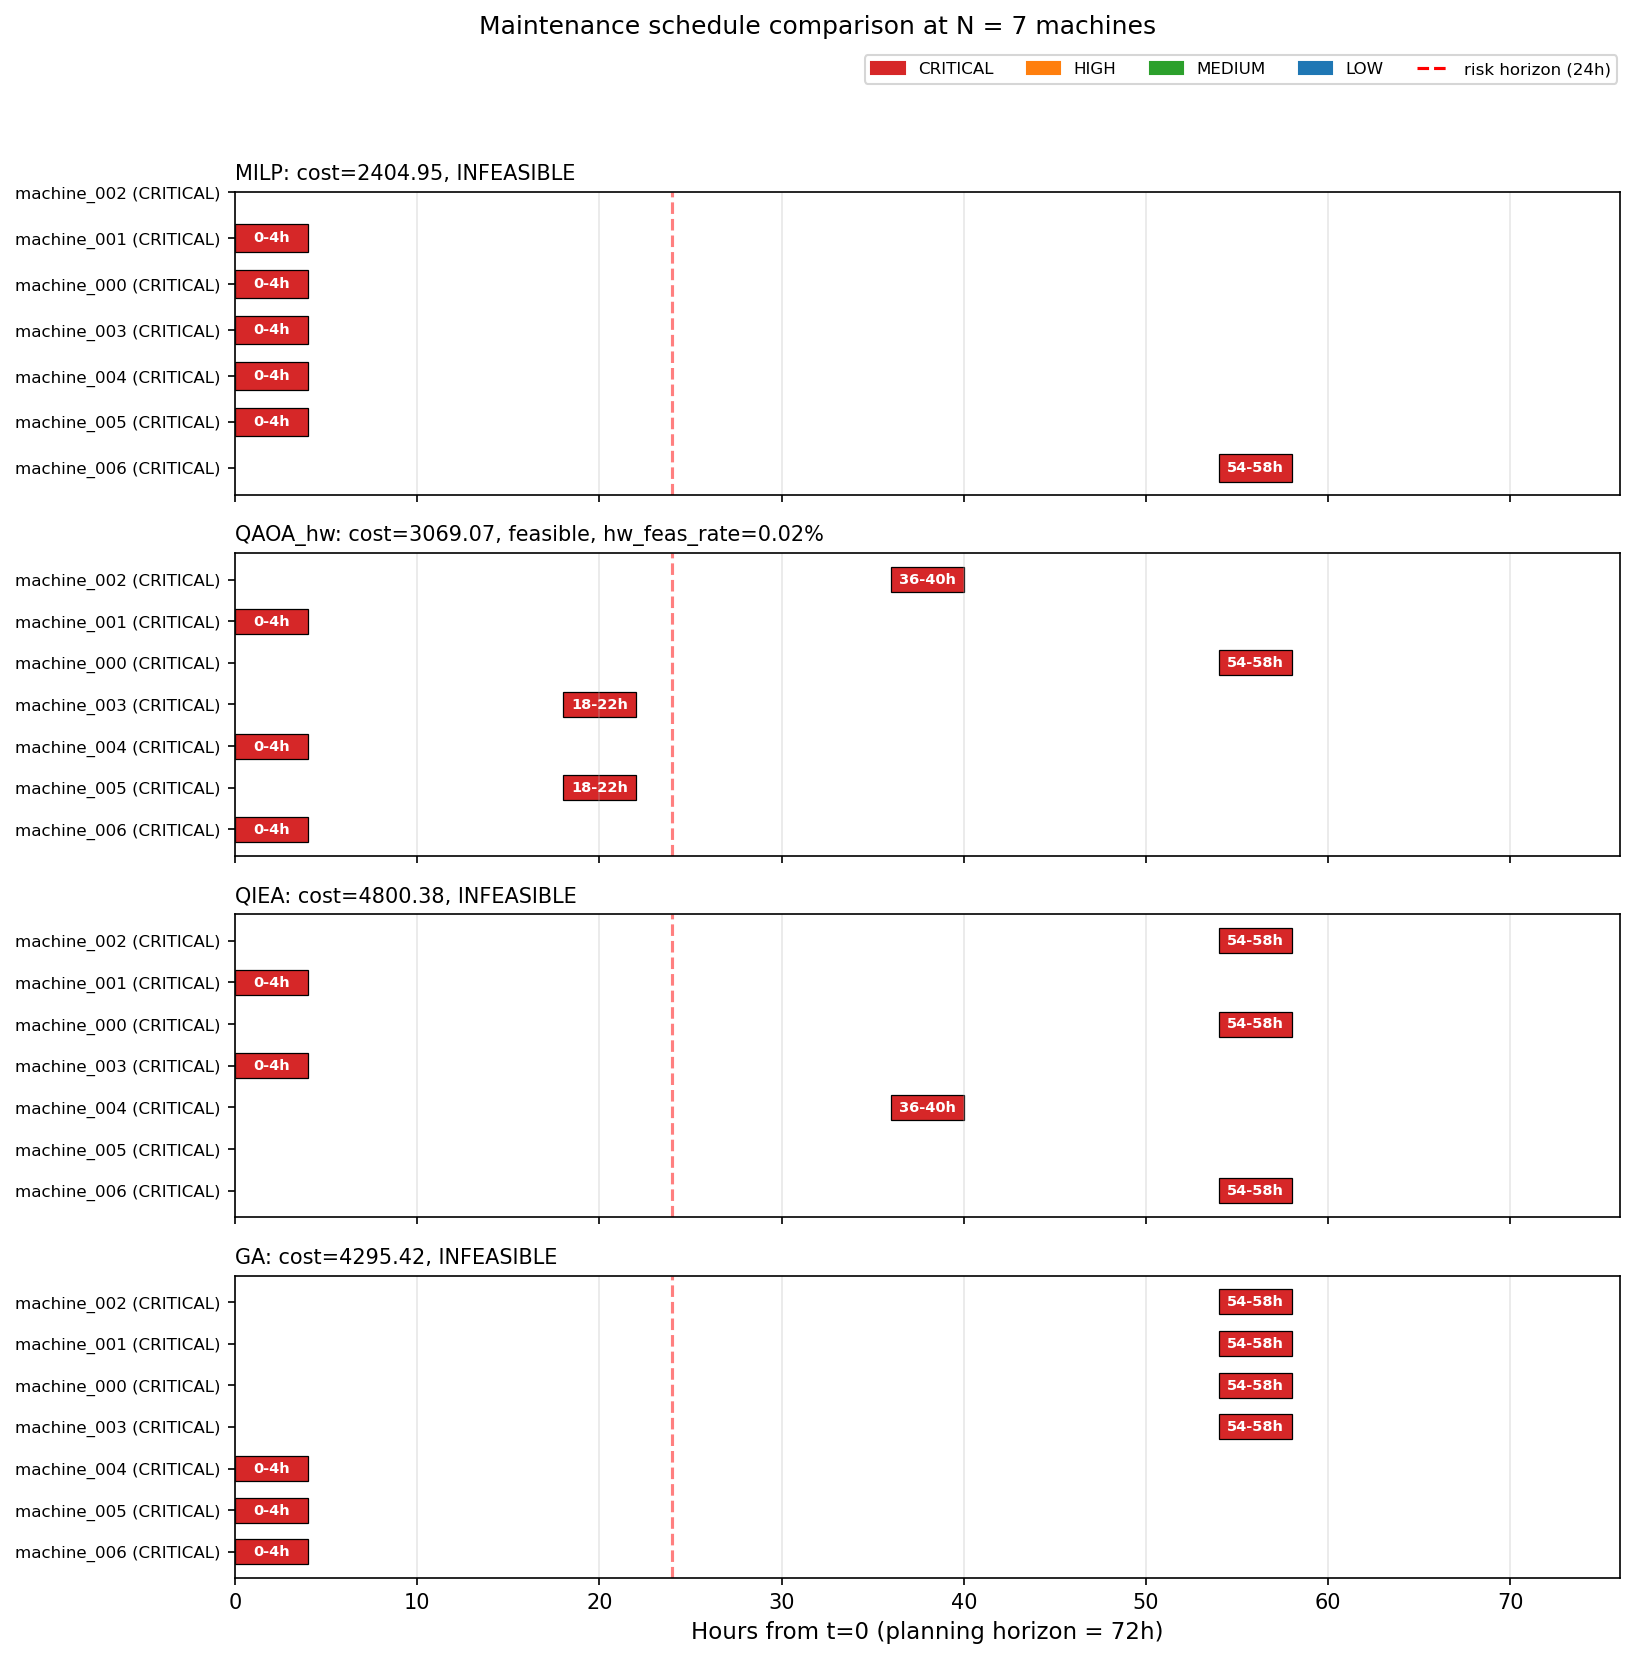
\includegraphics[width=0.95\textwidth]{figures/images/extended_gantt_N7.png}
    \caption{Decoded maintenance schedules at $N=7$ from MILP,
    \textbf{QAOA-XY on \texttt{ibm\_fez} (measured)}, QIEA, and GA.
    The vertical red dashed line marks the $24$-h risk horizon;
    bar colour encodes priority level
    (\textcolor{red}{CRITICAL}, \textcolor{orange}{HIGH},
    \textcolor{green!60!black}{MEDIUM},
    \textcolor{blue}{LOW}); each bar is the $4$-hour
    maintenance window. Every bar to the right of the red line is
    a (C3) violation. QAOA-XY incurs only $2$ risk-horizon
    violations (\texttt{machine\_002} at $h=36$ and
    \texttt{machine\_000} at $h=54$) compared with $V=8$ for the
    best classical heuristic.}
    \label{fig:extended_gantt_n7}
\end{figure}
\FloatBarrier

\subsection{Synthesis: Recent Advances Adapted to Our Problem}
\label{sec:synthesis}

Two literature streams informed our constraint-native quantum approach.

\textbf{IWS-QAOA} \cite{Niroula2026} embeds a warm-started XY-mixer Hamiltonian in a classical loop that iteratively refines bias from prior samples and applies greedy steepest-descent repair (see also \cite{Magann2025,Singh2025} for related warm-start formulations). Adapted to our streaming-derived $N=3$ instance (greedy warm-start biases the XY-mixer initial state, four iterations at $p=2$ refine $(\gamma,\beta)$ via COBYLA), the IWS-QAOA simulator recovers the MILP optimum (cost $300.00$, $31$~s); since greedy is already optimal at this scale, QAOA layers serve as a verifier — same role as the hardware match in Section~\ref{sec:complex_streaming}.

\textbf{Reverse-annealing SQA with pause} \cite{PerezArmas2024} uses a $4$-point schedule $[(0,1.0),(2.75,0.45),(82.75,0.45),(83.025,1.0)]$ holding the system at $\Gamma=0.45$ for an $80\,\mu$s tunnelling pause. Adapted to our PIMC SQA (16 replicas seeded from greedy with $10\%$ random flips; ramp $\Gamma$ $0.05\to0.45$, hold $120$ sweeps, ramp back to $0.01$), the streaming $N=4$ instance reaches low QUBO energy ($-30{,}706.4$) but no one-hot-feasible schedule: inter-replica coupling at low $\Gamma$ pulls replicas to the same near-feasible minimum. Reported here as a negative result; the template is better suited to D-Wave hardware than simulator.

Both adaptations confirm the basic QAOA-XY hardware result: productive quantum methods for constrained scheduling \emph{preserve constraint structure by construction} (XY-ring mixer, projector-Hamiltonian initial state) rather than translating constraints to QUBO penalties.

\subsection{Conditions for a Quantum or Quantum-Inspired Advantage}
For the basic-constraint formulation, MILP/CBC dominates every quantum and QI method up to $N=150$. For the complex-constraint streaming formulation at $N=5$ (MILP structurally infeasible), QAOA-XY hardware is the only solver returning a usable schedule, at cost only $1.3\%$ above MILP best-effort; classical alternatives either fail feasibility or pay $2.6\times$ cost premium. Operationally meaningful quantum advantage therefore requires both (i) constraint-native architecture (XY-ring mixer or equivalent) and (ii) constraint-tight regime where exact methods break. Mapping the empirical boundary at larger $N$, additional backends, and richer constraints (crew routing, machine dependencies, non-linear damage-recovery) is future work (Chapter~7).

Chapter~7 synthesises these findings with contributions from Chapters~3--5 and lists framework-wide limitations and future directions.
